%###############################################################################
\section{类模板}
%###############################################################################

%-----------------

\begin{frame}[fragile]{7.2~类模板}

类似函数模板,可以定义一个类模板用来生成具有\alert{相同结构}的一族类实例:

\vspace{-4mm}

\begin{columns}[t]

\column{0.65\textwidth}
\begin{blueblock}{\texttt{Array}类模板定义}
\begin{lstlisting}[moreemph={T}]
template<typename T, size_t N>
class Array {
    T m_ele[N];
public:
    Array() {}
    Array(const std::initializer_list<T> &);
    T& operator[](size_t i);
    constexpr size_t size() { return N; }
};
\end{lstlisting}
\end{blueblock}

\column{0.3\textwidth}
\begin{yellowblock}{说明}
$\bullet$ 类型参数\texttt{T}和非类型参数\texttt{N},分别用来表示元素的类型和元素的数目\\
$\bullet$ \alert{\texttt{initializer\_list}}~类型是C++11标准库提供的新类型,支持具有相同类型但数量未知的列表类型
\end{yellowblock}

\end{columns}

\end{frame}

%-----------------

%-------------------------------------
\subsection{成员函数定义}
%-------------------------------------

%-----------------

\begin{frame}[fragile]{7.2.1~成员函数定义}

与普通类相同,既可以在类的内部,也可以在\alert{类的外部}定义\alert{类模板成员函数}:

\vspace{-4mm}

\begin{columns}[t]

\column{0.65\textwidth}
\begin{blueblock}{\texttt{Array}类模板~构造函数~类外定义}
\begin{lstlisting}[moreemph={T,Array,initializer}]
template<typename T, size_t N>
Array<T, N>::Array(const std::initializer_list<T> &l):m_ele{T()}{
    size_t m = l.size() < N ? l.size() : N;
    for (size_t i = 0; i < m; ++i) {
        m_ele[i] = *(l.begin() + i);
    }
}
\end{lstlisting}
\end{blueblock}

\column{0.3\textwidth}
\begin{yellowblock}{说明}
$\bullet$ 必须以关键字\texttt{template}开始,后接\alert{与类模板相同}的模板参数列表\\
$\bullet$ 紧随类名后面的参数列表代表一个实例化的实参列表,每个参数不需要\texttt{typename}或\texttt{class}说明符
\end{yellowblock}

\end{columns}

\end{frame}

%-----------------

\begin{frame}[fragile]{7.2.1~成员函数定义}

与普通类相同,既可以在类的内部,也可以在\alert{类的外部}定义\alert{类模板成员函数}:

\vspace{-4mm}

\begin{columns}[t]

\column{0.65\textwidth}
\begin{blueblock}{\texttt{Array}类模板~构造函数~类外定义}
\vspace{-2mm}
\begin{lstlisting}[moreemph={T,Array,initializer}]
template<typename T, size_t N>
Array<T, N>::Array(const std::initializer_list<T> &l):m_ele{T()}{
    size_t m = l.size() < N ? l.size() : N;
    for (size_t i = 0; i < m; ++i) {
        m_ele[i] = *(l.begin() + i);
    }
}
\end{lstlisting}
\end{blueblock}
\begin{blueblock}<2->{\texttt{Array}类模板~\texttt{[]}运算符函数~类外定义}
\vspace{-2mm}
\begin{lstlisting}[moreemph={T,Array}]
template<typename T, size_t N>
T& Array<T, N>::operator[](size_t i) {
    return m_ele[i];
}
\end{lstlisting}
\end{blueblock}

\column{0.3\textwidth}
\begin{yellowblock}{说明}
$\bullet$ \texttt{m\_ele}中的每一个元素用T类型的默认初始化方式初始化\\
$\bullet$ 将形参\texttt{l}中的元素依次复制\\
$\bullet$ \texttt{l.begin}返回列表\texttt{l}中第一个元素的迭代器
\end{yellowblock}
\begin{yellowblock}<2->{说明}
类模板的下标运算符函数返回数组\texttt{m\_ele}中第\texttt{i}个元素的引用
\end{yellowblock}

\end{columns}

\end{frame}

%-----------------

%-------------------------------------
\subsection{实例化类模板}
%-------------------------------------

%-----------------

\begin{frame}[fragile]{7.2.2~实例化类模板}

当使用一个类模板时,我们需要\alert{显式}提供模板参数信息,即\alert{模板实参列表}:

\vspace{-4mm}

\begin{columns}[t]

\column{0.65\textwidth}
\begin{blueblock}{实例化\texttt{Array}类模板}
\begin{lstlisting}[moreemph={Array}]
Array<char, 5> a; //创建一个Array<char, 5>类型对象 a
Array<int, 5> b = {1,2,3}; //创建一个Array<int, 5>类型对象 b
\end{lstlisting}
\end{blueblock}
\uncover<2->{下面代码逐个输出对象\texttt{b}的每一个元素:}
\begin{blueblock}<2->{}
\begin{lstlisting}[moreemph={Array}]
for (int i = 0; i < b.size(); ++i)
    cout << b[i] << " ";
\end{lstlisting}
\end{blueblock}
\uncover<2->{输出结果为:\texttt{1 2 3 0 0}}

\column{0.3\textwidth}
\begin{yellowblock}{说明}
创建对象\texttt{b}时,将执行具有形参的构造函数,其形参\texttt{l}接受初始化列表 \texttt{\{1,2,3\}},其余元素具有默认值\texttt{0}
\end{yellowblock}


\end{columns}

\end{frame}

%-----------------

%-------------------------------------
\subsection{默认模板参数}
%-------------------------------------

%-----------------

\begin{frame}[fragile]{7.2.3~默认模板参数}

\alert{函数参数}可以具有默认值,\alert{模板参数}同样也可以有默认值:

\vspace{-4mm}

\begin{columns}[t]

\column{0.65\textwidth}
\begin{blueblock}{\texttt{Array}类模板定义二}
\vspace{-1mm}\begin{lstlisting}[moreemph={Array,T,Less,F}]
template<typename T = int, size_t N = 10>
class Array {
    // 其它成员保持不变
};
\end{lstlisting}\vspace{-1mm}
\end{blueblock}
\begin{blueblock}<2->{实例化\texttt{Array}类模板二}
\begin{lstlisting}[moreemph={Array}]
Array<> a = { 'A' };
cout << a.size() << " " << a[0] << endl;
\end{lstlisting}
\end{blueblock}
\uncover<2->{输出结果为:\texttt{10 65}}

\column{0.3\textwidth}
\begin{yellowblock}{说明}
$\bullet$ \alert{类模板参数}~\texttt{T}具有默认类型\texttt{int}\\
$\bullet$ \alert{类模板参数}~\texttt{N}具有默认值\texttt{10}
\end{yellowblock}
\begin{yellowblock}<2->{说明}
$\bullet$ \texttt{a}的元素数目为默认值\texttt{10}\\
$\bullet$ \texttt{a[0]}的类型为\texttt{int},字符\texttt{'A'}转换为\texttt{65}
\end{yellowblock}

\end{columns}

\end{frame}

%-----------------

\begin{frame}[fragile]{7.2.3~默认模板参数}

为\alert{函数模板参数}提供默认值:

\vspace{-4mm}

\begin{columns}[t]

\column{0.65\textwidth}
\begin{blueblock}{\texttt{Array}类模板定义三}
\vspace{-2mm}\begin{lstlisting}[moreemph={Array,T,Less,F}]
template<typename T, size_t N = 10>
class Array {
    // 其它成员保持不变
public:
    template<typename F = Less<T>>
    void sort(F f = F());
};
\end{lstlisting}\vspace{-2mm}
\end{blueblock}
\begin{blueblock}<2->{\texttt{Less}类模板定义}
\vspace{-2mm}\begin{lstlisting}[moreemph={Less,T}]
template<typename T>
struct Less{
    bool operator()(const T &a, const T &b) {
        return a < b;
    }
};
\end{lstlisting}\vspace{-2mm}
\end{blueblock}

\column{0.3\textwidth}
\begin{yellowblock}{说明}
$\bullet$ 新增了一个成员函数模板\texttt{sort},用来对数组进行排序\\
$\bullet$ \texttt{sort}的\alert{函数模板参数}~\texttt{F}具有默认值\texttt{Less<T>}
\end{yellowblock}
\begin{yellowblock}<2->{说明}
类模板\texttt{Less<T>}具有一个模板参数\texttt{T},且只有一个函数调用运算符,该成员函数带有两个形参,用来比较两个形参的大小,返回值类型为\texttt{bool}
\end{yellowblock}

\end{columns}

\end{frame}

%-----------------

\begin{frame}[fragile]{7.2.3~默认模板参数}

和\alert{类模板参数}一样,\alert{函数模板参数}也可以有默认值:

\vspace{-4mm}

\begin{columns}[t]

\column{0.65\textwidth}
\begin{blueblock}{\texttt{Array}类模板定义三}
\vspace{-1mm}\begin{lstlisting}[moreemph={Array,T,Less,F}]
template<typename T, size_t N = 10>
class Array {
    // 其它成员保持不变
public:
    template<typename F = Less<T>>
    void sort(F f = F());
};
\end{lstlisting}\vspace{-1mm}
\end{blueblock}

\column{0.3\textwidth}
\begin{yellowblock}{说明}
$\bullet$ \texttt{sort}的\alert{函数参数}~\texttt{f}也有默认值,即\texttt{F}类的一个函数对象,代表默认比较方式为\texttt{Less}
\end{yellowblock}
\begin{greenblock}<2->{问题}
理清~\alert{函数参数}和\alert{模板参数}的概念
\end{greenblock}

\end{columns}

\end{frame}

%-----------------

%###############################################################################
\section{排序与查找}
%###############################################################################

%-------------------------------------
\subsection{排序算法}
%-------------------------------------

%-----------------

\begin{frame}[fragile]{7.3.1~排序算法}

排序是数据处理的最基本任务,目的是按照某种规则将一组无序数据重新排列,使之有序。

\vspace{-4mm}
\begin{columns}[t]

\column{0.65\textwidth}
\begin{blueblock}<2->{\texttt{Array}类模板定义四}
\vspace{-3mm}
\begin{lstlisting}[moreemph={Array,T}]
template<typename T, size_t N>
class Array {
public:
    template<typename F = Less<T> >
    void selectionSort(F f = F());      //选择排序
    template<typename F = Less<T> >
    void insertionSort(F f = F());      //插入排序
    template<typename F = Less<T> >
    void bubbleSort(F f = F());         //冒泡排序
private:
    void swap(int i, int j){
        T t = m_ele[i];
        m_ele[i] = m_ele[j];
        m_ele[j] = t;
    }
};
\end{lstlisting}
\vspace{-1mm}
\end{blueblock}

\column{0.3\textwidth}
\begin{yellowblock}<2->{说明}
成员\texttt{swap}函数用来交换两个元素的位置,它仅在\texttt{Array}类内部使用,因此它的访问属性为\texttt{private}
\end{yellowblock}

\end{columns}

\end{frame}

%-----------------

\begin{frame}[fragile]{7.3.1 排序算法\normalsize{~---~选择排序}}

每次在待排序元素中选择最小的一个,换放到已排序数列后面

\vspace{1mm}

\begin{center}
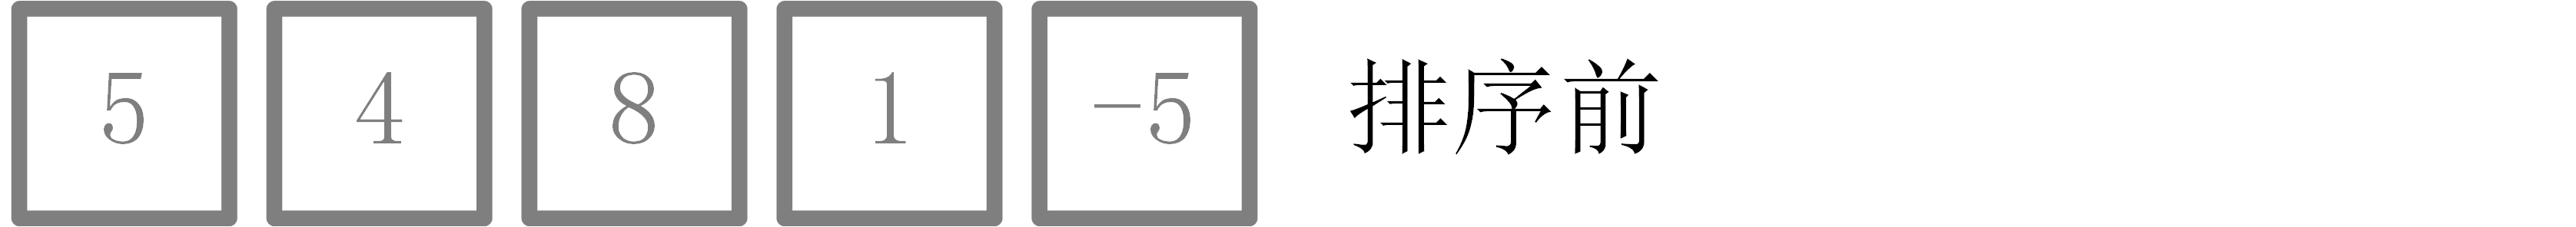
\includegraphics[width=0.8\textwidth]{selection_sort_1}\\\vspace{3mm}
\uncover<2->{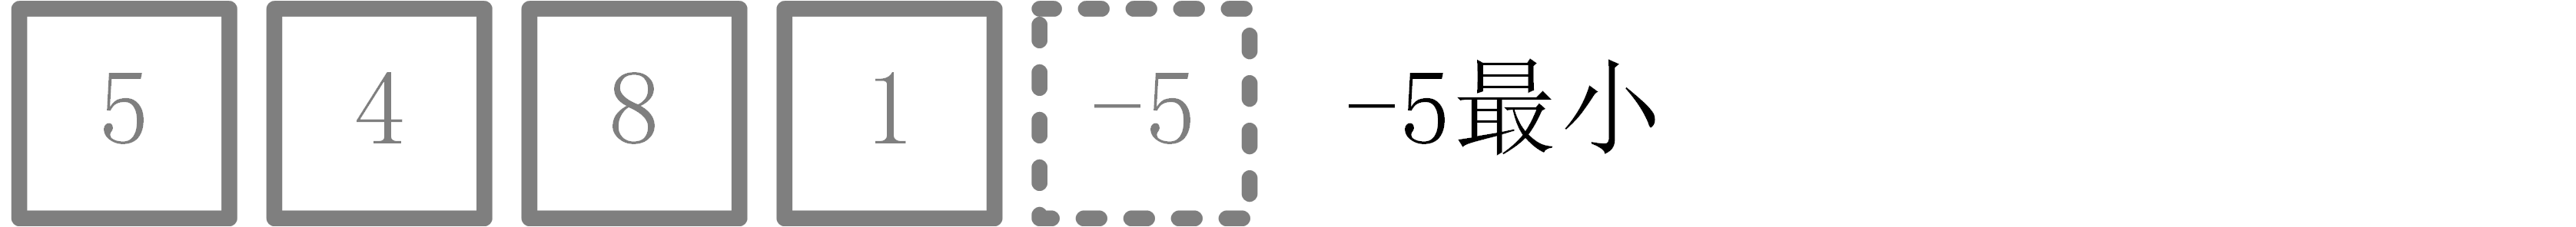
\includegraphics[width=0.8\textwidth]{selection_sort_2}}\\\vspace{-11mm}
\uncover<3->{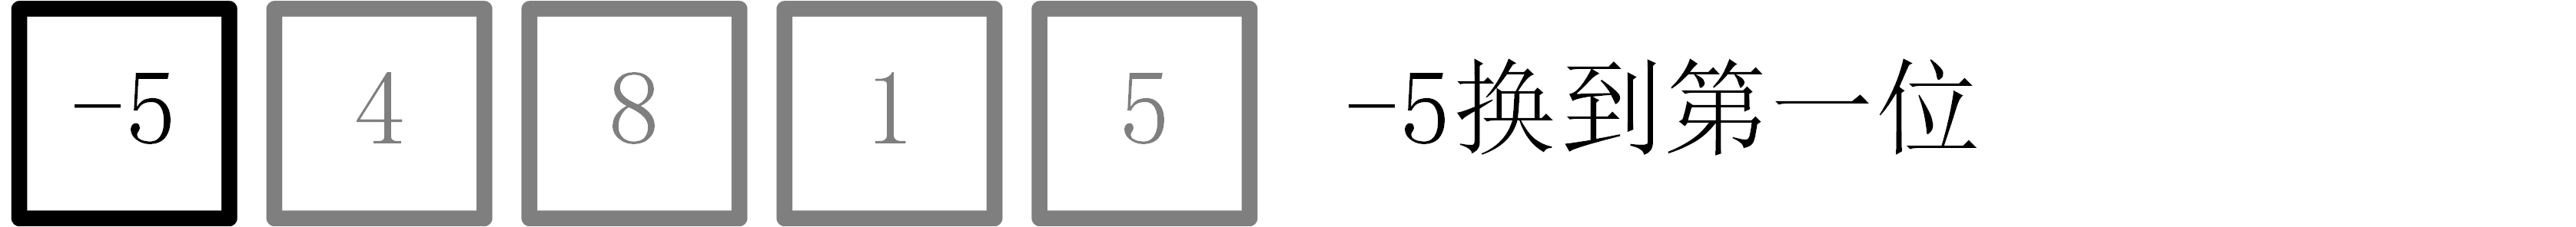
\includegraphics[width=0.8\textwidth]{selection_sort_3}}\\
\uncover<4->{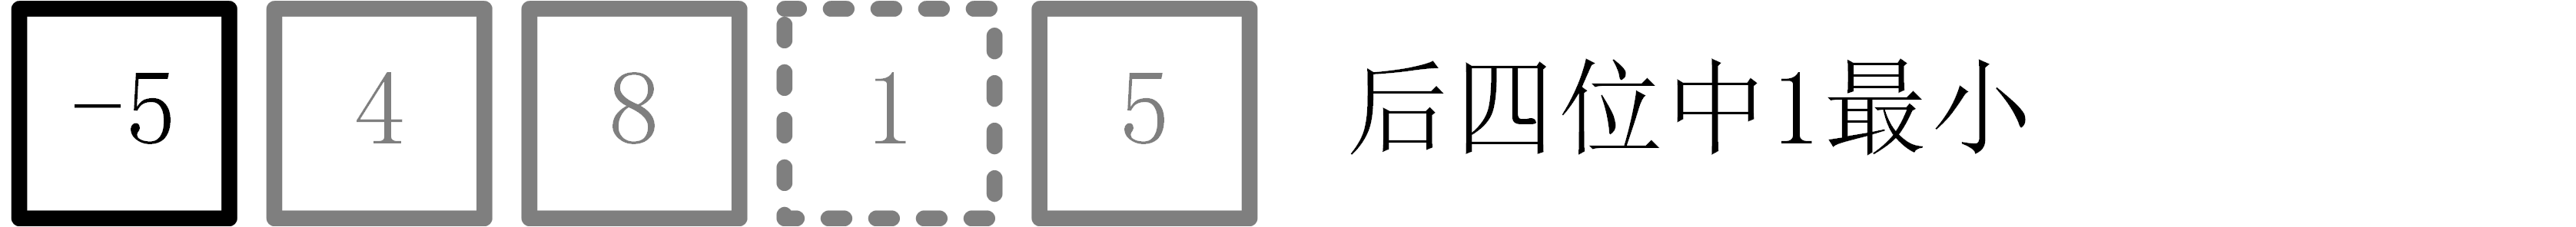
\includegraphics[width=0.8\textwidth]{selection_sort_4}}\\\vspace{-11mm}
\uncover<5->{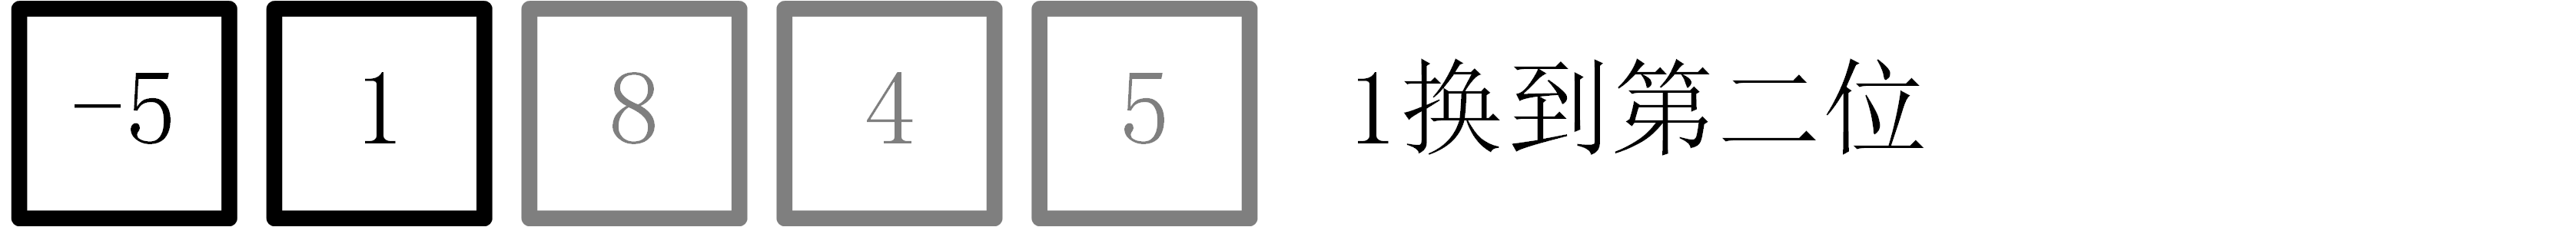
\includegraphics[width=0.8\textwidth]{selection_sort_5}}\\
\uncover<6->{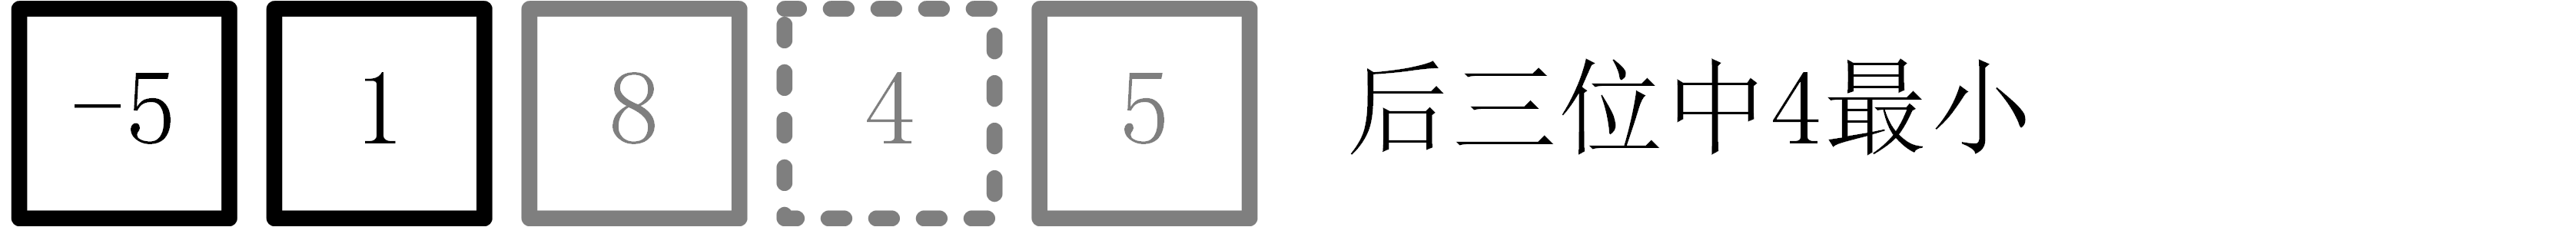
\includegraphics[width=0.8\textwidth]{selection_sort_6}}\\\vspace{-11mm}
\uncover<7->{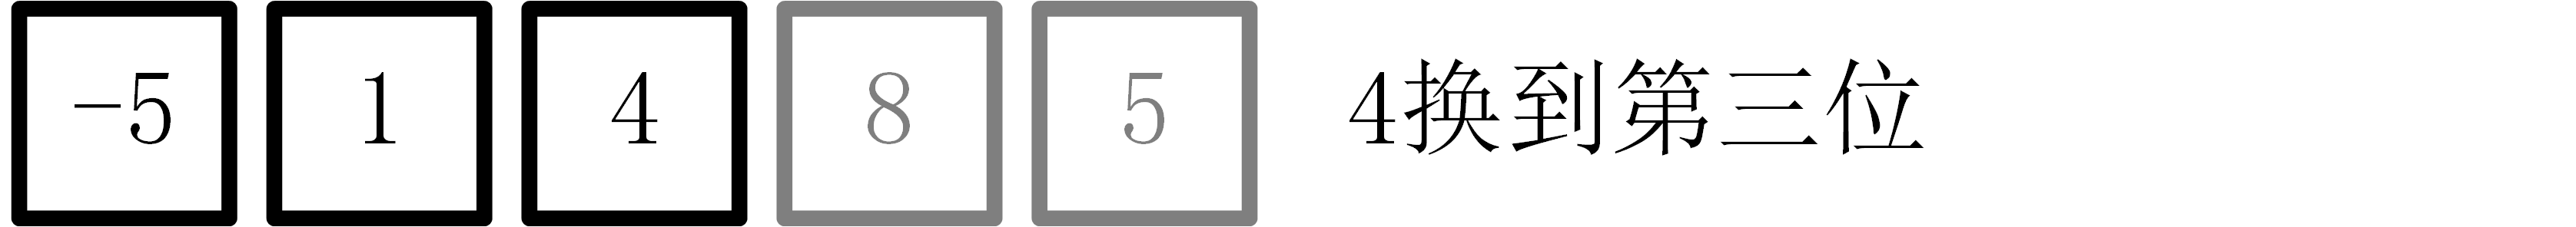
\includegraphics[width=0.8\textwidth]{selection_sort_7}}\\
\uncover<8->{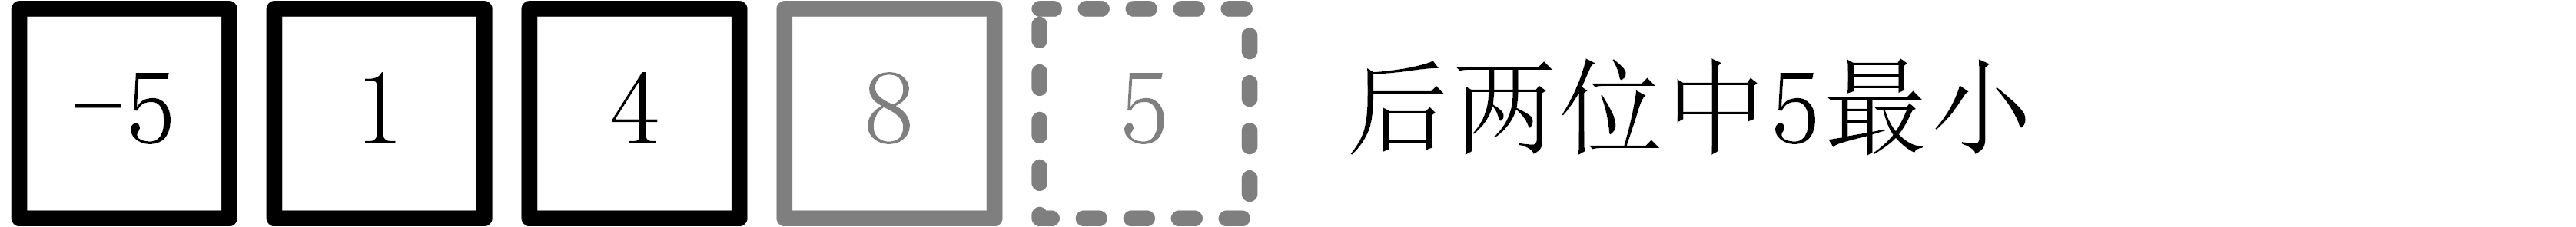
\includegraphics[width=0.8\textwidth]{selection_sort_8}}\\\vspace{-11mm}
\uncover<9->{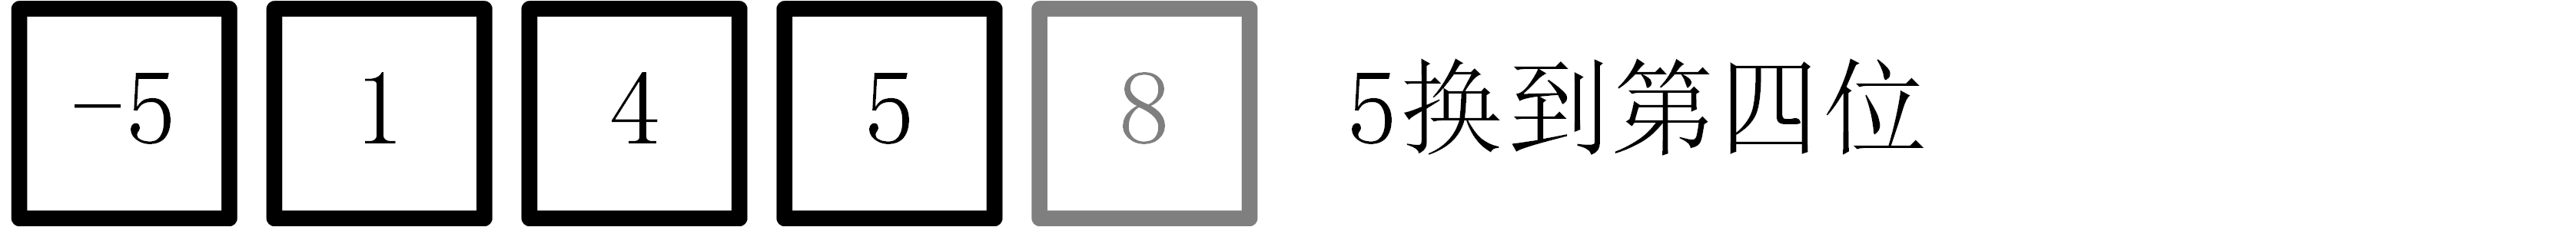
\includegraphics[width=0.8\textwidth]{selection_sort_9}}\\
\uncover<10->{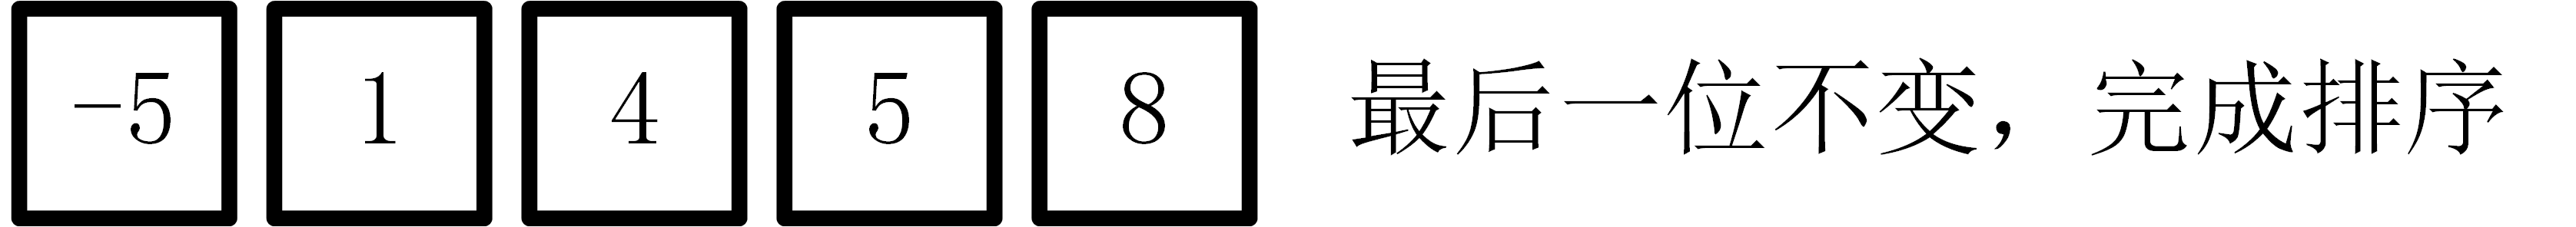
\includegraphics[width=0.8\textwidth]{selection_sort_10}}
\end{center}

\end{frame}

%-----------------

\begin{frame}[fragile]{7.3.1 排序算法\normalsize{~---~选择排序}}

选择排序算法的实现如下:

\vspace{-4mm}

\begin{columns}[t]

\column{0.65\textwidth}
\begin{blueblock}{\texttt{Array}成员函数\texttt{selectionSort}定义}
\begin{lstlisting}[moreemph={Array,T,F}]
template<typename T, size_t N>
template<typename F >
void Array<T, N>::selectionSort(F f) {
    for (int i = 0; i < N - 1; ++i){
        int min = i;        // 记录待排序数据中最小元素位置
        for (int j = i + 1; j < N; ++j) {
            if (f(m_ele[j], m_ele[min]))
                min = j;    //更新最小元素位置
        }
        swap(i, min);       //把最小元素放到位置i
    }
}
\end{lstlisting}
\end{blueblock}

\column{0.3\textwidth}
\begin{yellowblock}{说明}
\texttt{if}语句里的条件表达式将调用函数对象\texttt{f}(\texttt{Less<T>}),检查第一个实参对象是否小于第二个实参对象
\end{yellowblock}

\end{columns}

\end{frame}

%-----------------

\begin{frame}[fragile]{7.3.1 排序算法\normalsize{~---~插入排序}}

将待排序的元素逐个插入已经排好序的元素序列中

\vspace{1mm}

\begin{center}
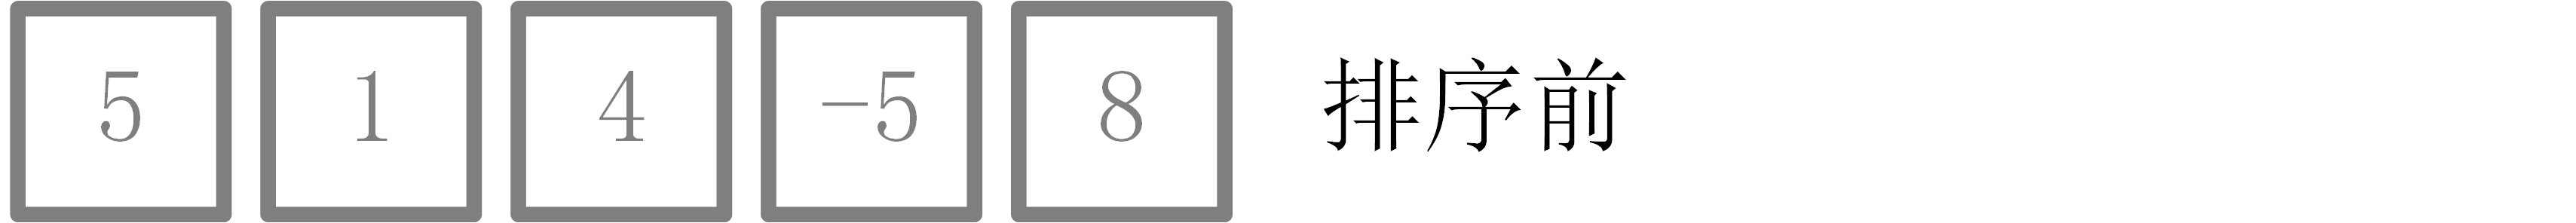
\includegraphics[width=0.8\textwidth]{insertion_sort_1}\\\vspace{3mm}
\uncover<2->{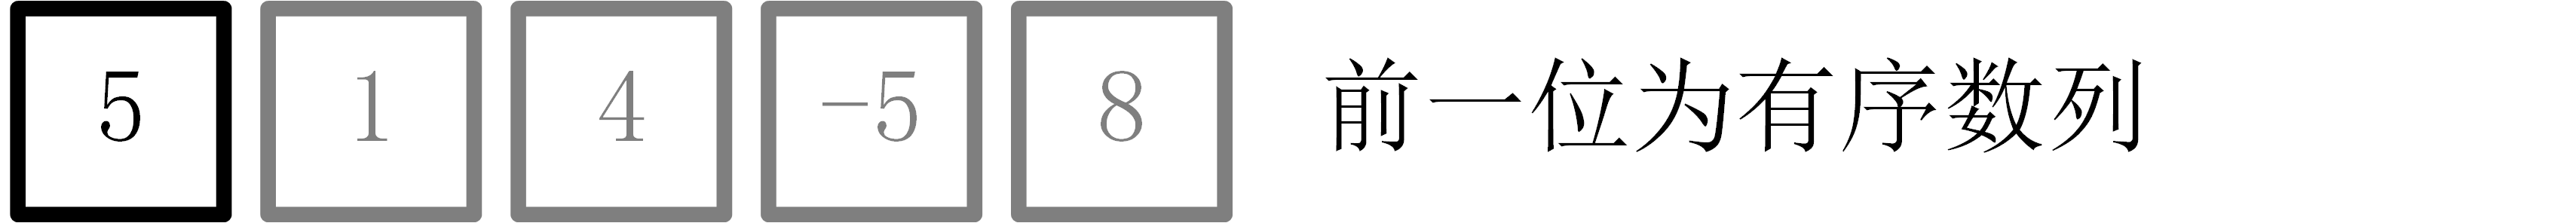
\includegraphics[width=0.8\textwidth]{insertion_sort_2}}\\
\uncover<3->{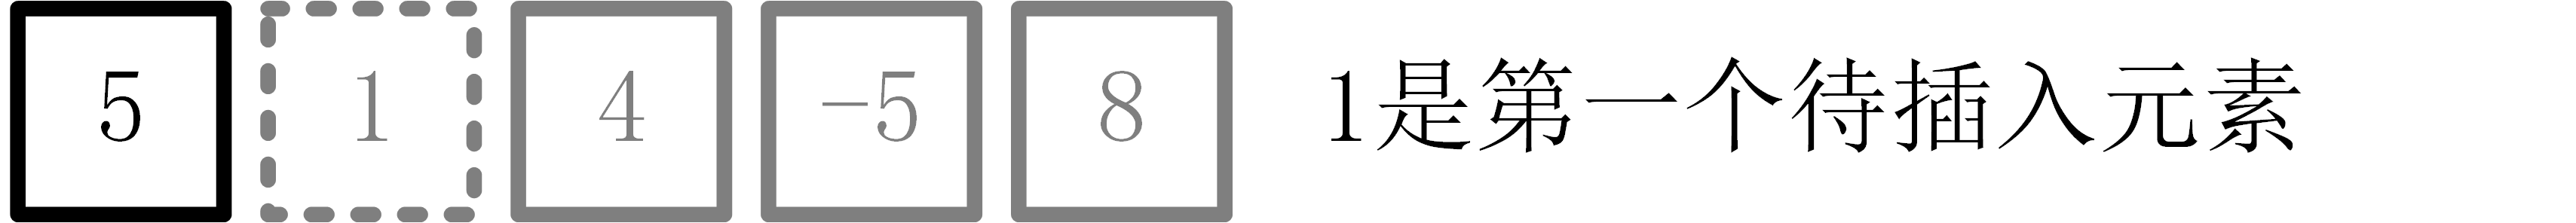
\includegraphics[width=0.8\textwidth]{insertion_sort_3}}\\\vspace{-10.9mm}
\uncover<4->{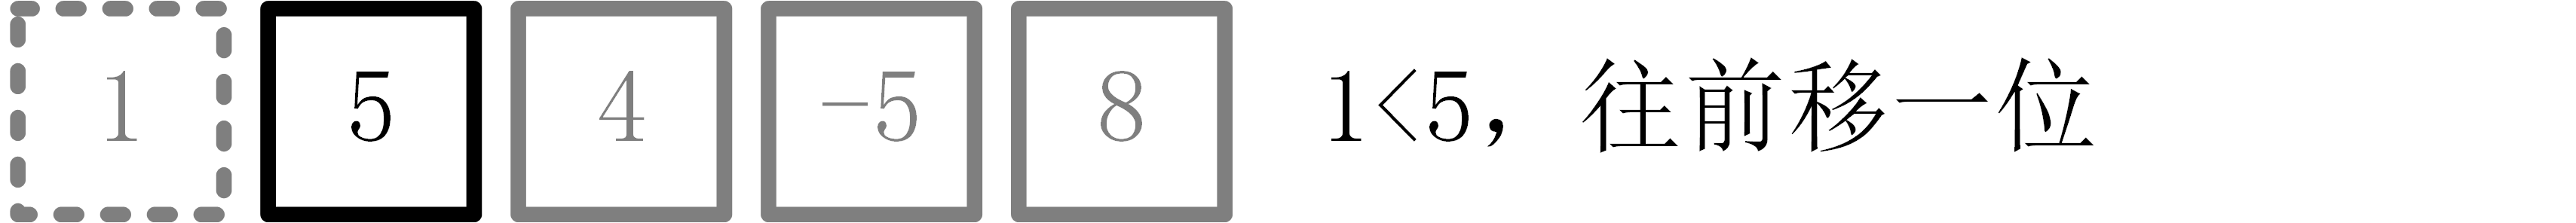
\includegraphics[width=0.8\textwidth]{insertion_sort_4}}\\\vspace{-10.9mm}
\uncover<5->{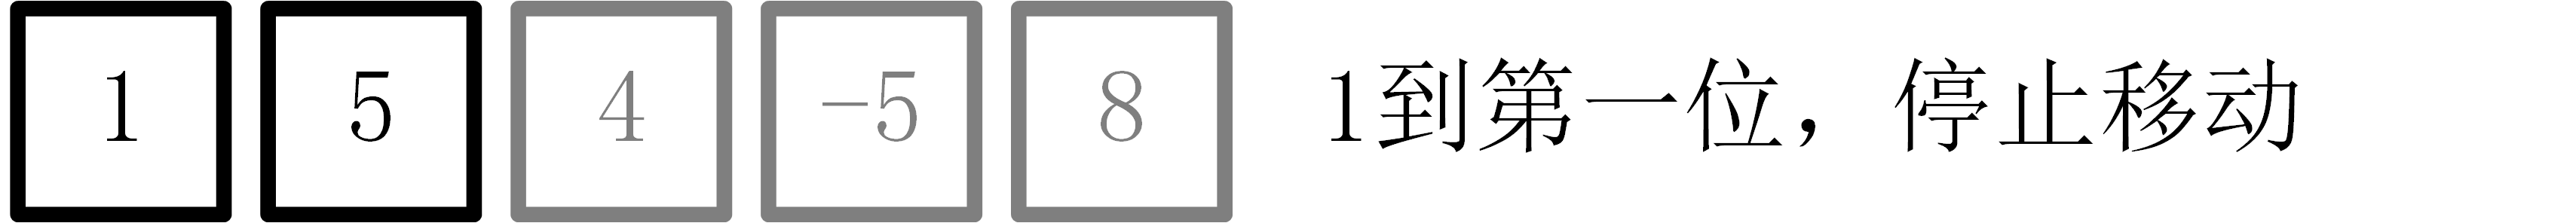
\includegraphics[width=0.8\textwidth]{insertion_sort_5}}\\
\uncover<6->{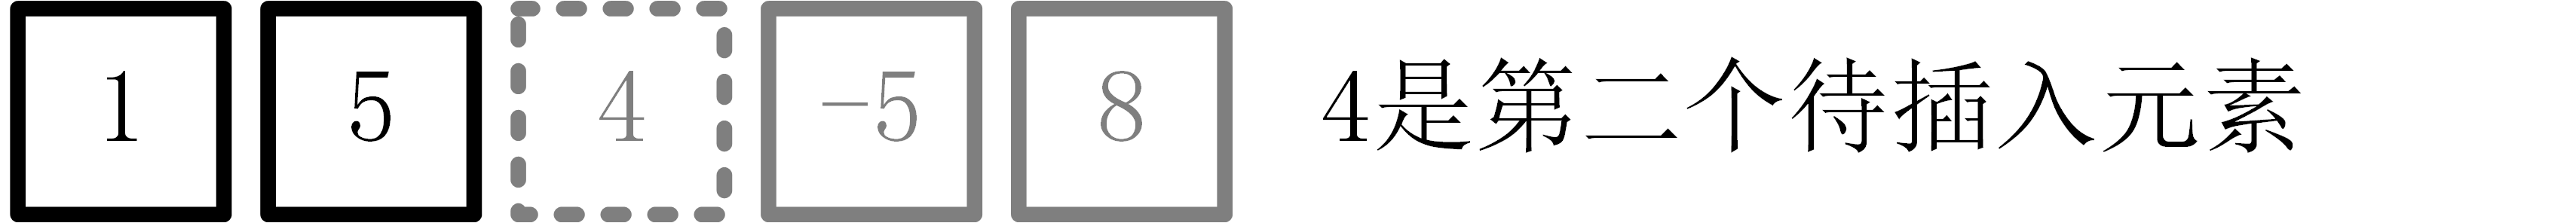
\includegraphics[width=0.8\textwidth]{insertion_sort_6}}\\\vspace{-10.9mm}
\uncover<7->{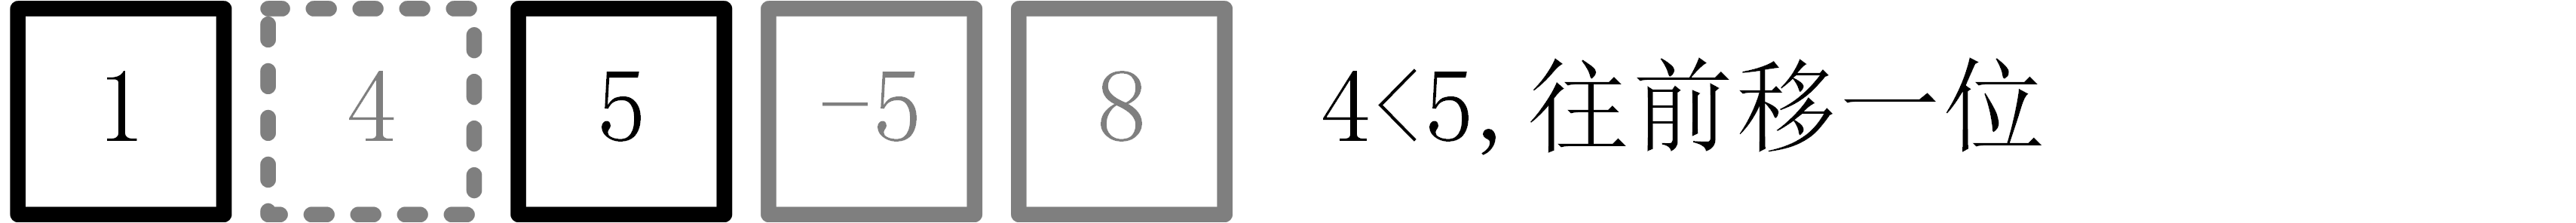
\includegraphics[width=0.8\textwidth]{insertion_sort_7}}\\\vspace{-10.9mm}
\uncover<8->{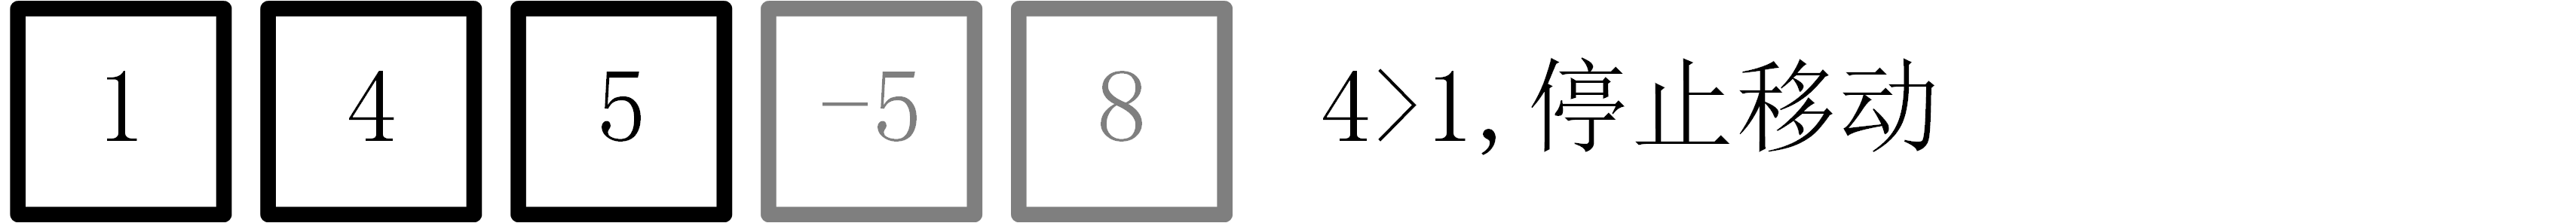
\includegraphics[width=0.8\textwidth]{insertion_sort_8}}\\
\uncover<9->{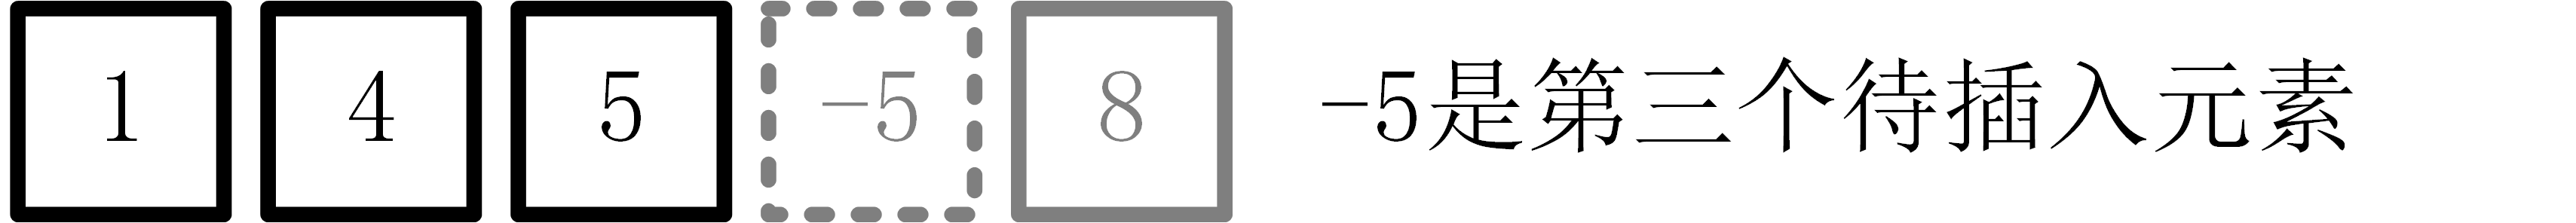
\includegraphics[width=0.8\textwidth]{insertion_sort_9}}\\\vspace{-10.9mm}
\uncover<10->{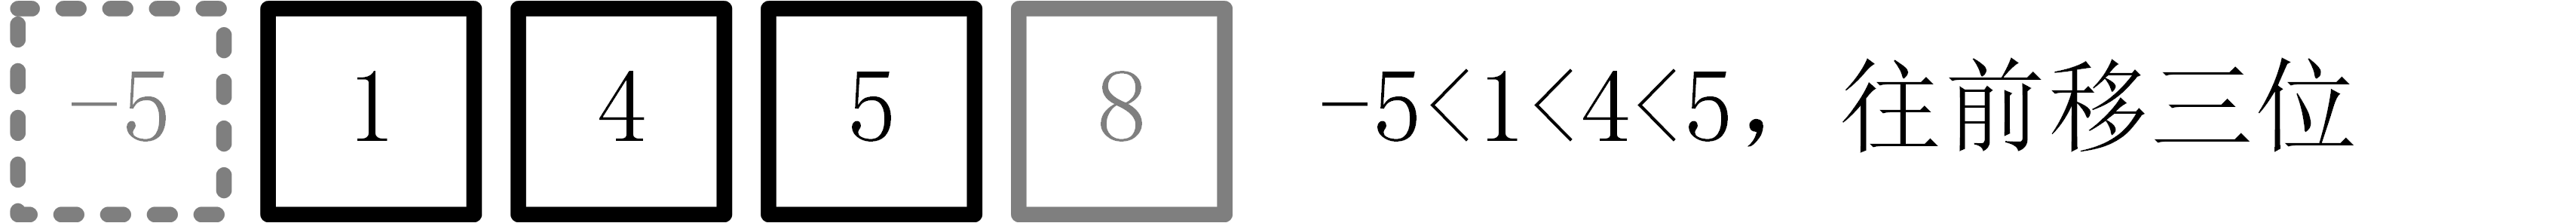
\includegraphics[width=0.8\textwidth]{insertion_sort_10}}\\\vspace{-10.9mm}
\uncover<11->{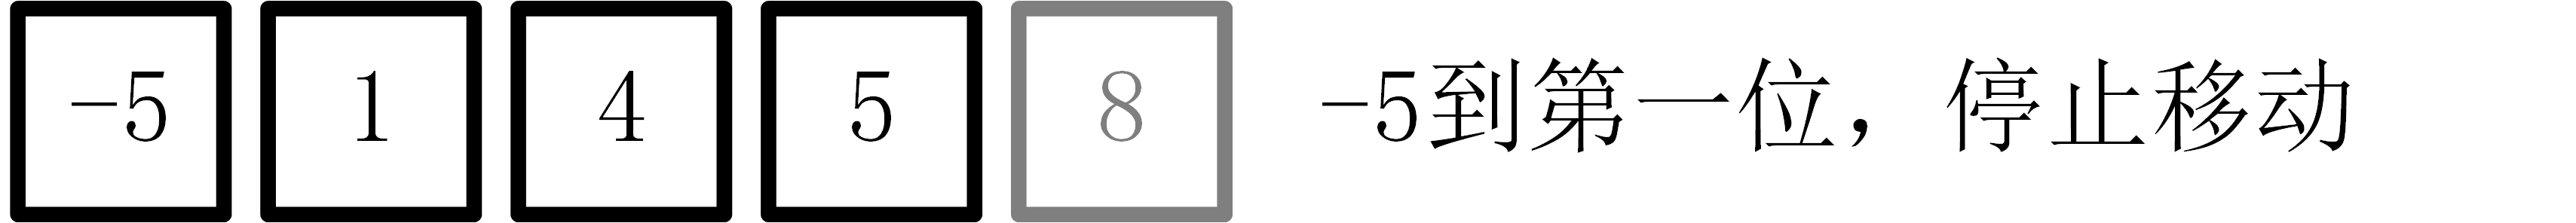
\includegraphics[width=0.8\textwidth]{insertion_sort_11}}\\\vspace{1mm}
\uncover<12->{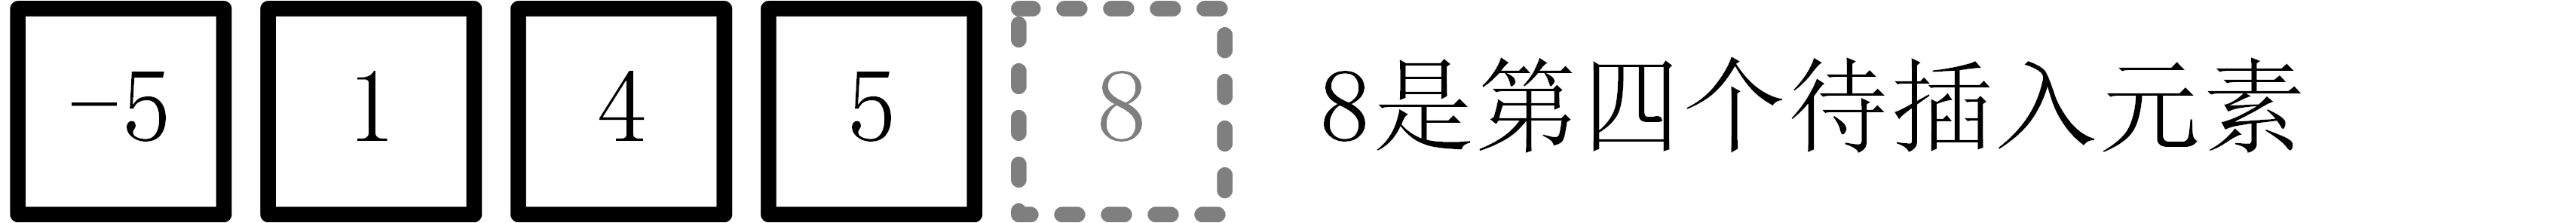
\includegraphics[width=0.8\textwidth]{insertion_sort_12}}\\\vspace{-10.8mm}
\uncover<13->{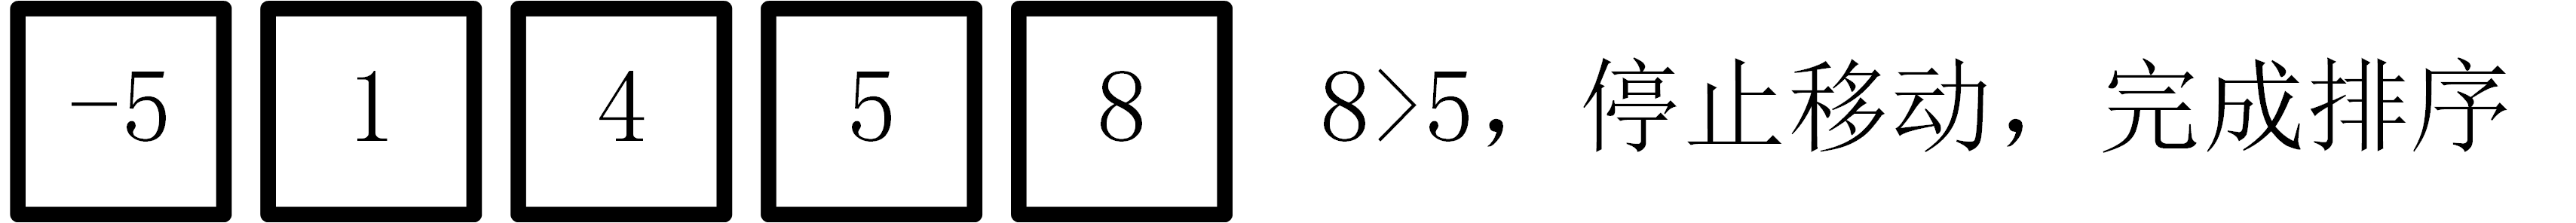
\includegraphics[width=0.8\textwidth]{insertion_sort_13}}
\end{center}

\end{frame}

%-----------------

\begin{frame}[fragile]{7.3.1 排序算法\normalsize{~---~插入排序}}

插入排序算法的实现如下:

\vspace{-4mm}

\begin{columns}[t]

\column{0.65\textwidth}
\begin{blueblock}{\texttt{Array}成员函数\texttt{insertionSort}定义}
\begin{lstlisting}[moreemph={Array,T,F}]
template<typename T, size_t N>
template<typename F >
void Array<T, N>::insertionSort(F f) {
    for (int i = 1, j; i < N; ++i) {
        T t = m_ele[i];                 //待插入元素
        for (j = i; j > 0; --j) {       //查找插入位置
            if (f(m_ele[j - 1], t))
                break;
            m_ele[j] = m_ele[j - 1];    //逐个向后移动元素
        }
        m_ele[j] = t;                   //将待插入元素放到正确位置
    }
}
\end{lstlisting}
\end{blueblock}

\column{0.3\textwidth}

\end{columns}

\end{frame}

%-----------------

\begin{frame}[fragile]{7.3.1 排序算法\normalsize{~---~冒泡排序}}

不断比较相邻的两个元素,如果发现逆序则交换

\vspace{1mm}

\begin{center}
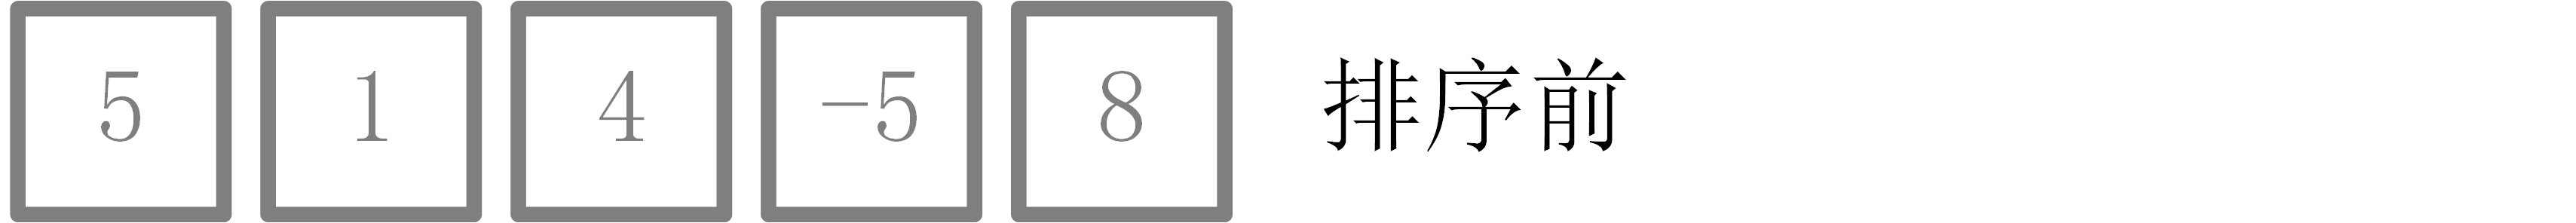
\includegraphics[width=0.8\textwidth]{bubble_sort_1}\\\vspace{3mm}
\uncover<2->{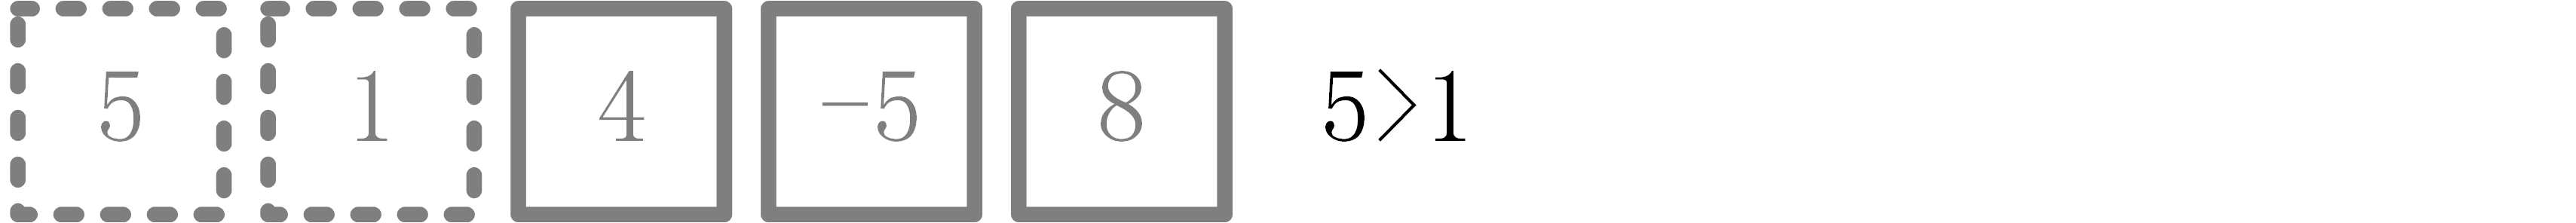
\includegraphics[width=0.8\textwidth]{bubble_sort_2}}\\\vspace{-10.9mm}
\uncover<3->{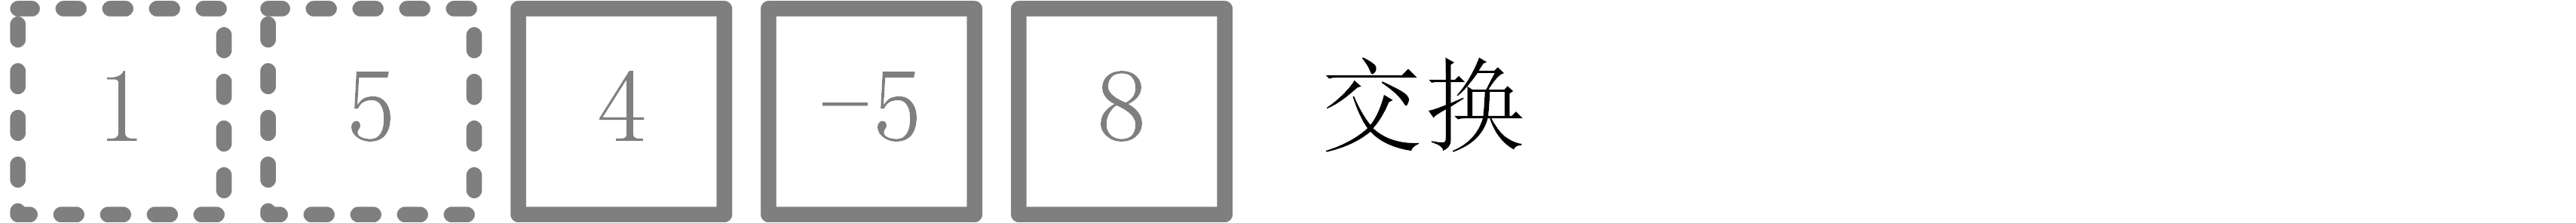
\includegraphics[width=0.8\textwidth]{bubble_sort_3}}\\
\uncover<4->{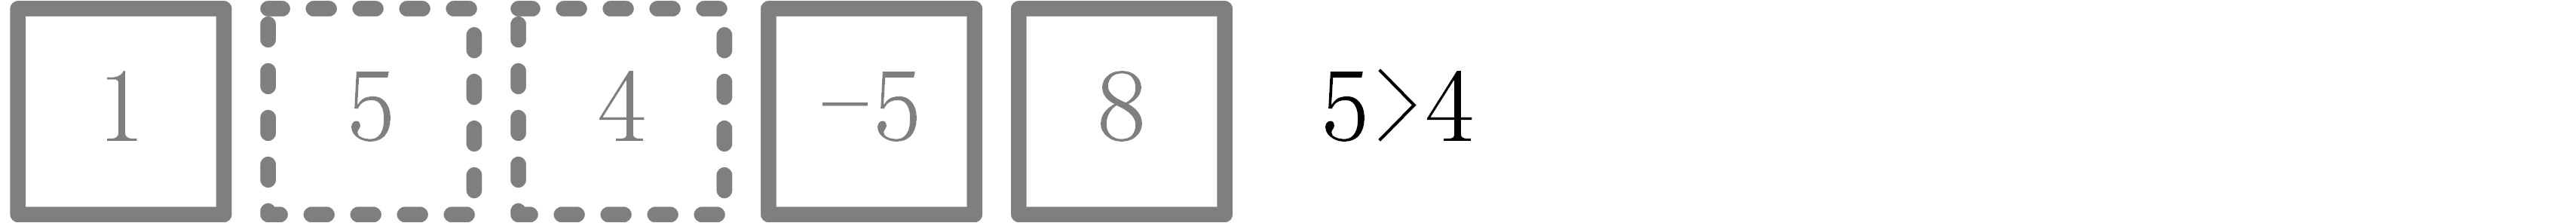
\includegraphics[width=0.8\textwidth]{bubble_sort_4}}\\\vspace{-10.9mm}
\uncover<5->{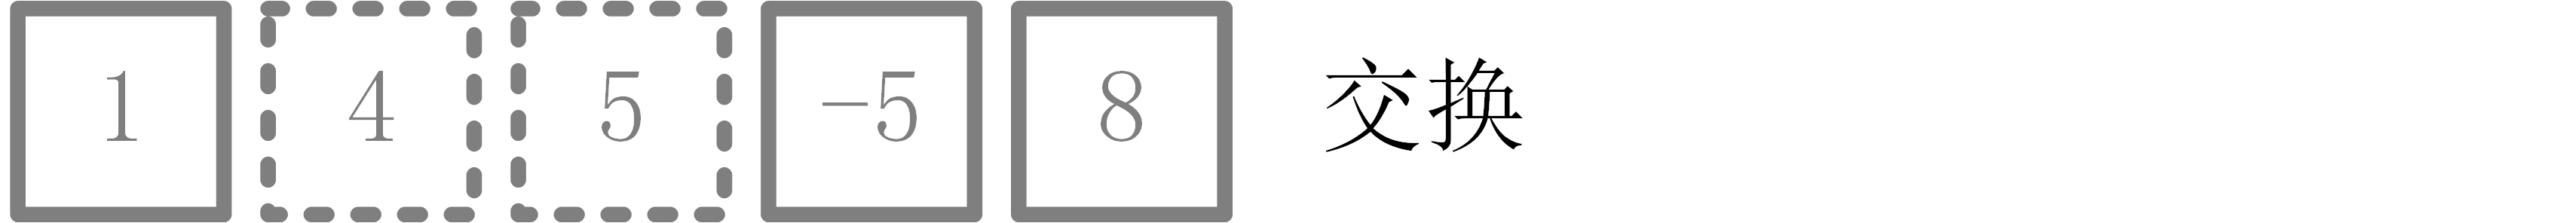
\includegraphics[width=0.8\textwidth]{bubble_sort_5}}\\
\uncover<6->{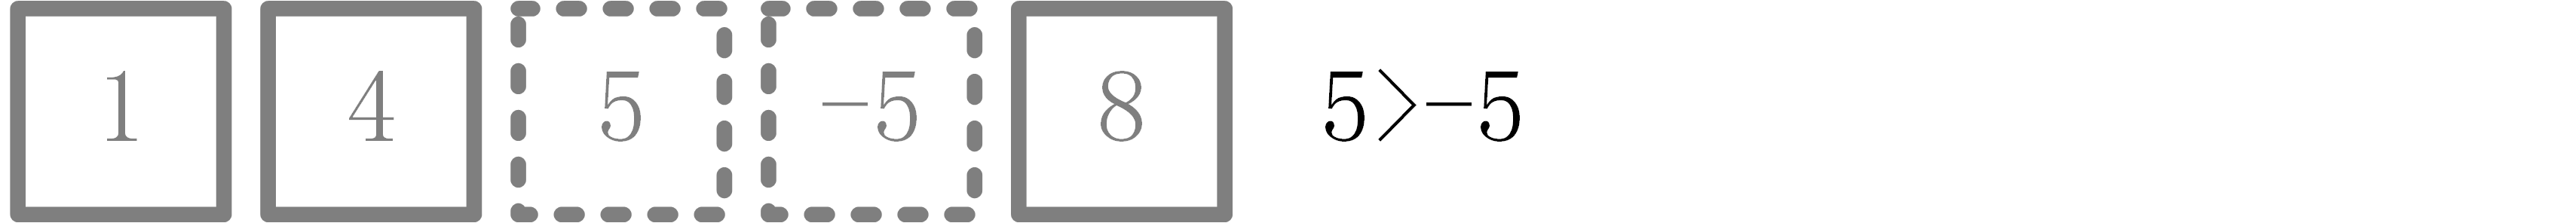
\includegraphics[width=0.8\textwidth]{bubble_sort_6}}\\\vspace{-10.9mm}
\uncover<7->{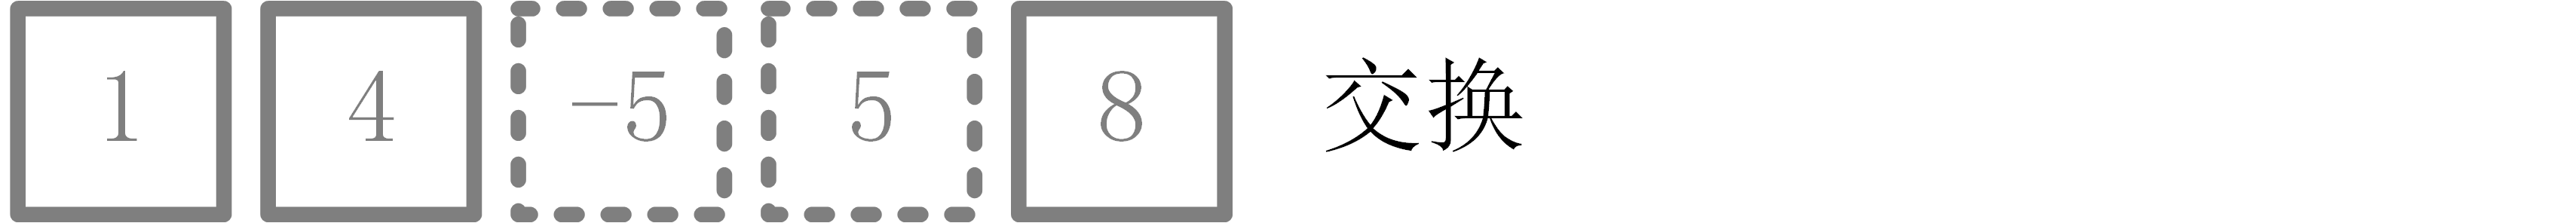
\includegraphics[width=0.8\textwidth]{bubble_sort_7}}\\
\uncover<8->{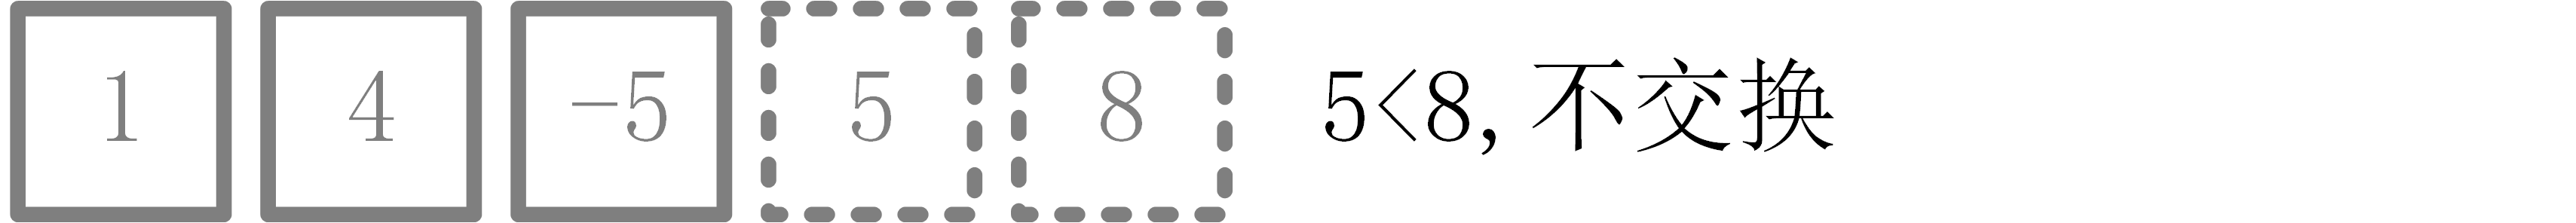
\includegraphics[width=0.8\textwidth]{bubble_sort_8}}\\\vspace{1mm}
\uncover<9->{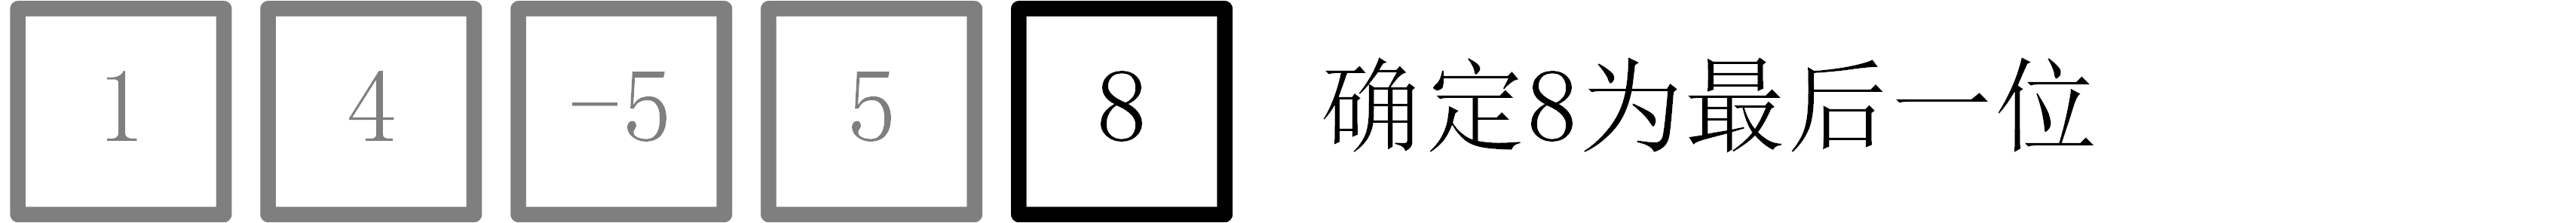
\includegraphics[width=0.8\textwidth]{bubble_sort_9}}
\end{center}

\end{frame}

%-----------------

\begin{frame}[fragile]{7.3.1 排序算法\normalsize{~---~冒泡排序}}

冒泡排序算法的实现如下:

\vspace{-4mm}

\begin{columns}[t]

\column{0.65\textwidth}
\begin{blueblock}{\texttt{Array}成员函数\texttt{selectionSort}定义}
\begin{lstlisting}[moreemph={Array,T,F}]
template<typename T, size_t N>
template<typename F >
void Array<T, N>::bubbleSort(F f){
    for (int i = N - 1; i >= 0; --i){
        for (int j = 0; j <= i - 1; ++j){
            if (f(m_ele[j + 1], m_ele[j]))
                swap(j, j + 1); //相邻元素交换
        }
    }
}
\end{lstlisting}
\end{blueblock}

\column{0.3\textwidth}

\end{columns}

\end{frame}

%-----------------

\begin{frame}[fragile]{7.3.1 排序算法\normalsize{~---~快速排序}}

\begin{block}<1->{快速排序}
 快速排序是冒泡排序的改进,在排序过程中数据移动少。\\
\end{block}
\begin{block}<2->{快速排序的基本思想}
基本思想:划分和分治递归。\\
   \begin{enumerate}
     \item 划分:将整个数组划分为两个部分,第一部分所有值小于基准值(key),第二部分所以值大于基准值(key)。(基准值的选择是随机的,一般选择待排数组的第一个元素)。
     \item 分治递归:第一步将数组划分为两部分后,两部分内部还不是有序的,再分别对两部分递归地进行快速排序,最终得到一个完整的有序数组
   \end{enumerate}
\end{block}
\end{frame}

\begin{frame}[fragile]{7.3.1 快速排序}

\begin{block}{快速排序的流程}
(1)left、right指针(索引)分别指向待排数组的首、尾。\\
(2)left 指针向后遍历,right指针向前遍历。\\
(3)当right指针指向元素小于基准值(key)时,right指针元素便赋值给left指针元素,完成转移。\\
(4)当left指针指向元素大于基准值(key)时,left指针元素便赋值给right指针元素,完成转移。\\
(5)最终当left=right时,遍历结束。\\
(6)以基准值(key)为界限,把数组分成两部分,分别对这两部分进行快速排序(显然这是一个递归的过程)\\
\end{block}

\end{frame}
\begin{frame}[fragile]{7.3.1 快速排序}
\begin{center}
 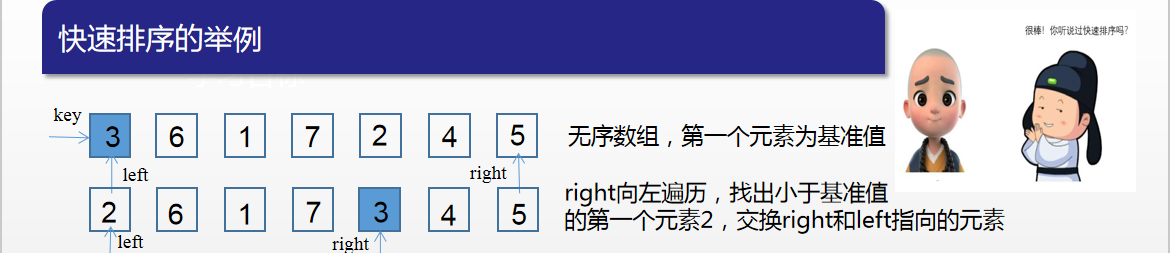
\includegraphics[scale=0.38]{quick_sort_1.png}\\
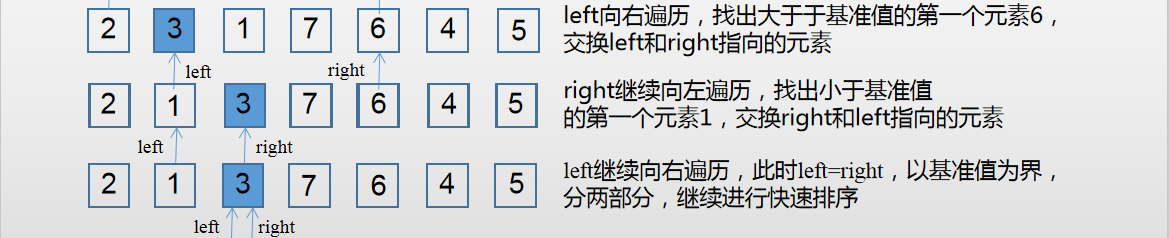
\includegraphics[scale=0.38]{quick_sort_2.png}
\end{center}
\end{frame}
\begin{frame}[fragile]{7.3.1快速排序}
\begin{block}{快速排序的举例续}
\end{block}
\begin{center}
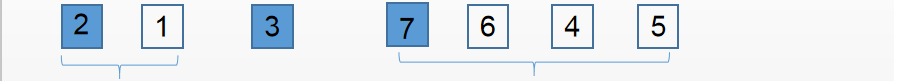
\includegraphics[scale=0.38]{quick_sort_6.png}
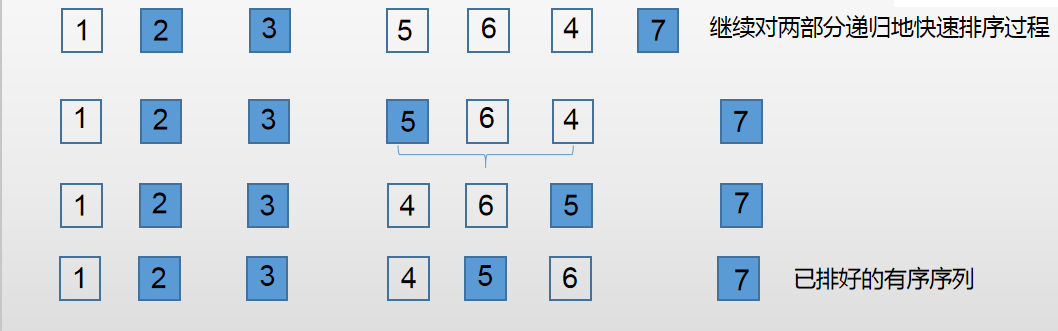
\includegraphics[scale=0.38]{quick_sort_7.png}
\end{center}
\end{frame}

%\begin{frame}[fragile]{7.3.1 快速排序}
%\begin{block}{快速排序的小技巧}
%(1)若以数组的第一个元素为基准值,则应该先用right向左遍历,然后再用left向右遍历。\\
%~\\
%(2)若以数组的最后一个元素为基准值,则应该先用left向右遍历,然后再用right向左遍历。\\
%~\\
%(3)一般不建议用数组中间的元素做基准值,但也可以用。\\
%~\\
%\end{block}
%
%\end{frame}
%\begin{frame}[fragile]{7.3.1 快速排序}
%~\\
%~\\
%\begin{center}
%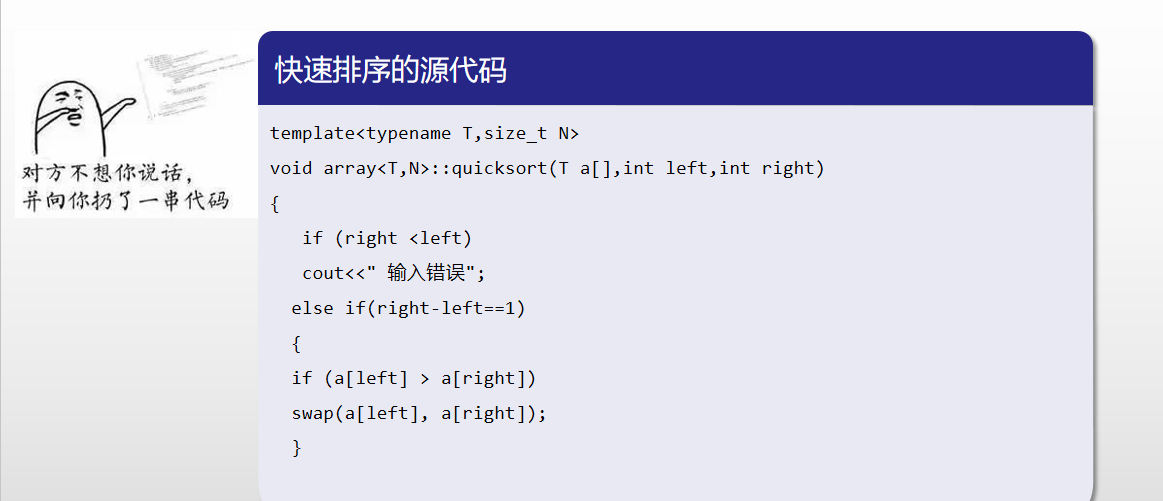
\includegraphics[scale=0.3]{quick_sort_3.png}
%\end{center}
%\end{frame}
%\begin{frame}[fragile]{7.3.1快速排序}
%~\\
%~\\
%\begin{center}
%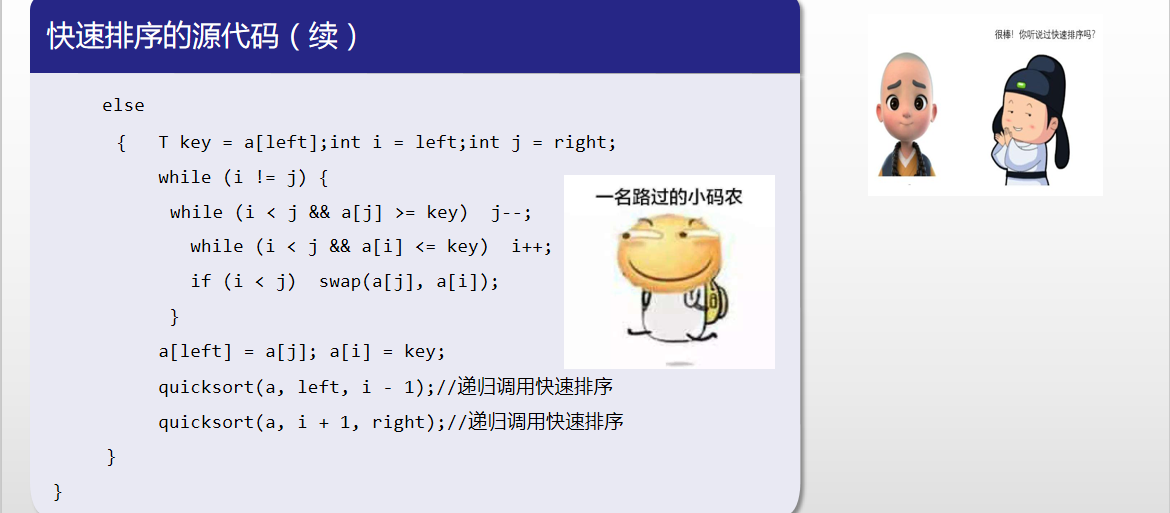
\includegraphics[scale=0.3]{quick_sort_4.png}
%\end{center}
%\end{frame}

\begin{frame}[fragile]{7.3.1 快速排序}
~\\
~\\
\begin{center}
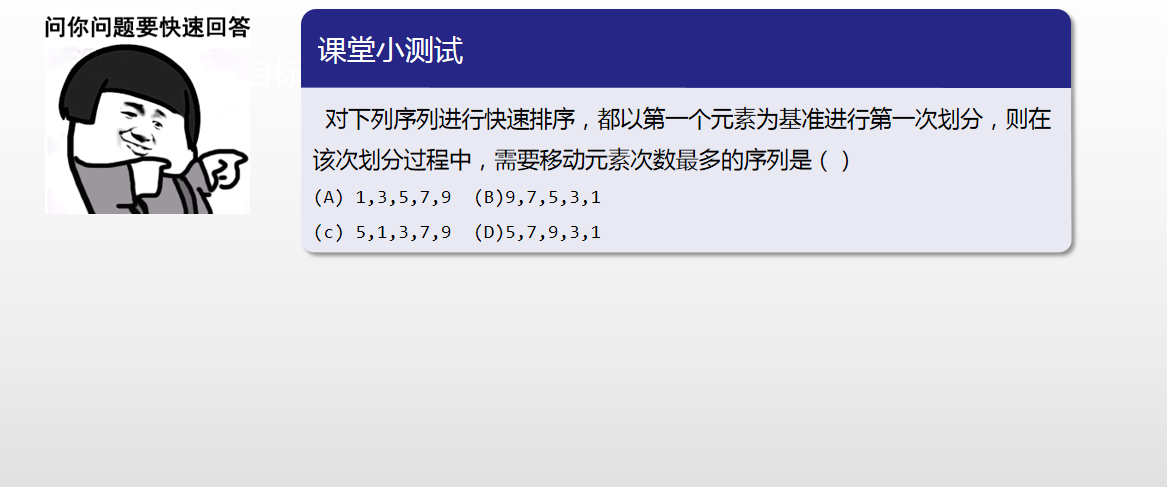
\includegraphics[scale=0.3]{quick_sort_5.png}
\end{center}
\end{frame}
%-----------------

\begin{frame}[fragile]{7.3.1 排序算法\normalsize{~---~快速排序}}

快速排序算法的实现如下:
\vspace{-4mm}
\begin{blueblock}{函数\texttt{quickSort}定义}
\begin{lstlisting}[moreemph={Array,T,F}]
template<typename T, size_t N>
template<typename F >
void Array<T, N>::quickSort(int left, int right, F f) {
	if (left < right){
		int i = left, j = right;
		T x = m_ele[left];
		while (i < j){
			while (i < j && f(x,m_ele[j])) j--;  // 从右向左找第一个小于x的数
			if (i < j)	m_ele[i++] = m_ele[j];
			while (i < j && f(m_ele[i],x))	i++; // 从左向右找第一个大于等于x的数
			if (i < j)	m_ele[j--] = m_ele[i];
		}
		m_ele[i] = x;
		quickSort(left, i - 1, f);             //左半部分排序
		quickSort(i + 1, right, f);           //右半部分排序
	}
}
\end{lstlisting}
\end{blueblock}

\end{frame}
%-------------------------------------
\subsection{二分查找算法}
%-------------------------------------

%-----------------

\begin{frame}[fragile]{7.3.2~二分查找算法}

又称折半查找,在有序序列中使用,其基本思想为分而治之

\vspace{1mm}

\begin{center}
\uncover<2->{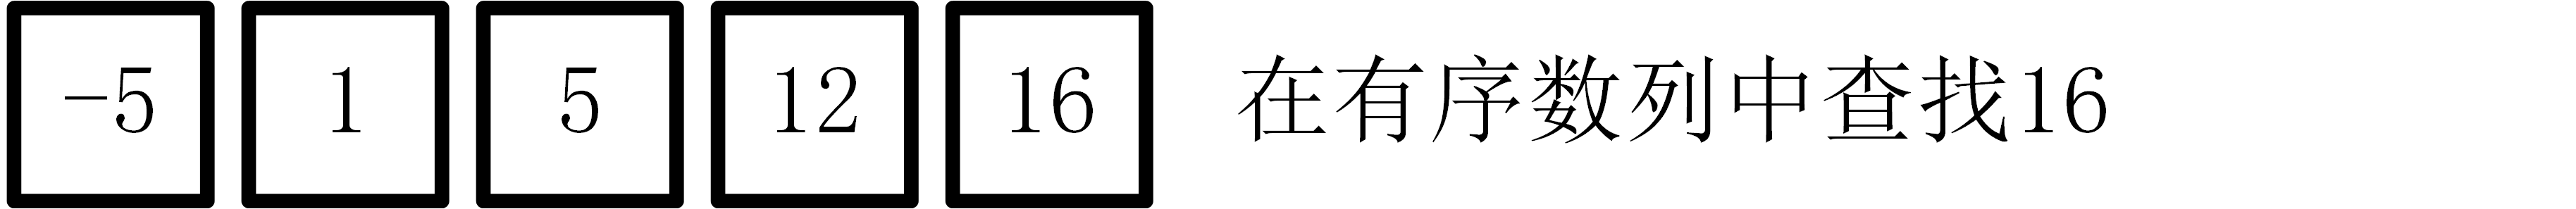
\includegraphics[width=0.8\textwidth]{binary_search_1}}\\\vspace{3mm}
\uncover<3->{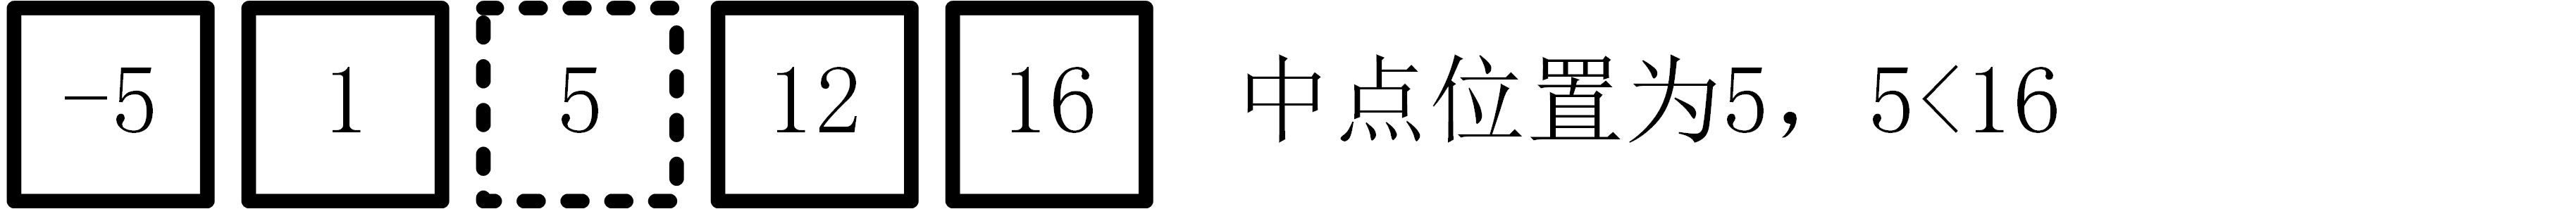
\includegraphics[width=0.8\textwidth]{binary_search_2}}\\\vspace{-10.1mm}
\uncover<4->{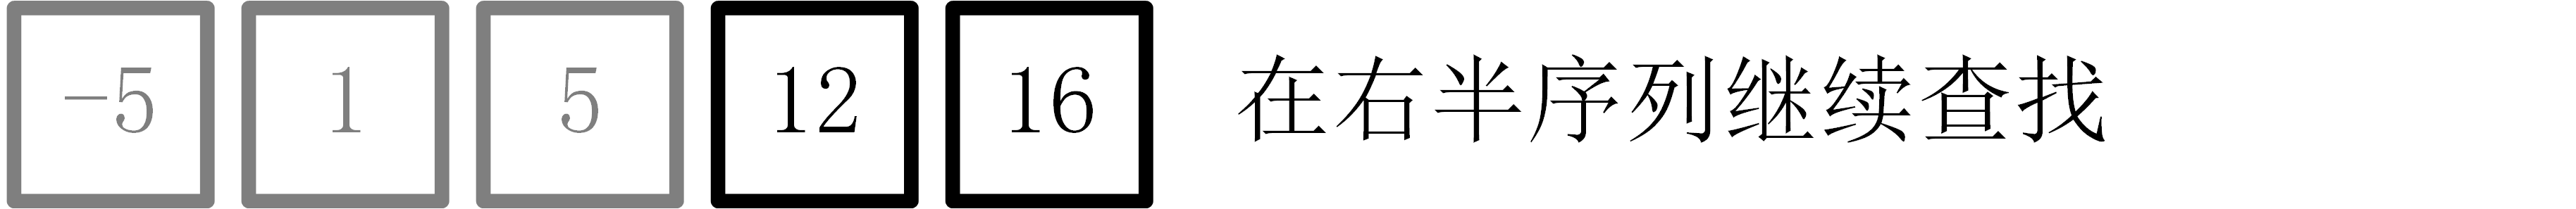
\includegraphics[width=0.8\textwidth]{binary_search_3}}\\\vspace{-10.1mm}
\uncover<5->{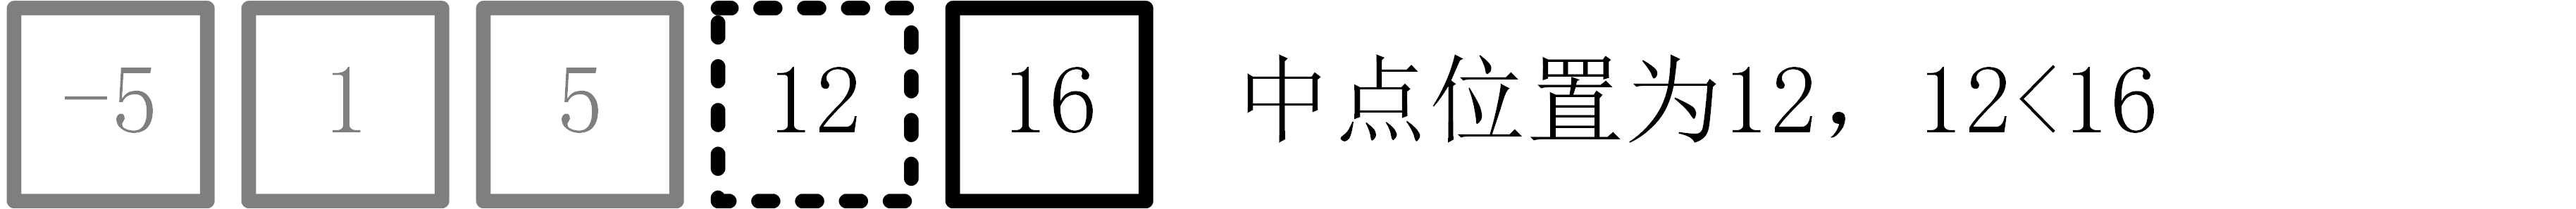
\includegraphics[width=0.8\textwidth]{binary_search_4}}\\\vspace{-10.1mm}
\uncover<6->{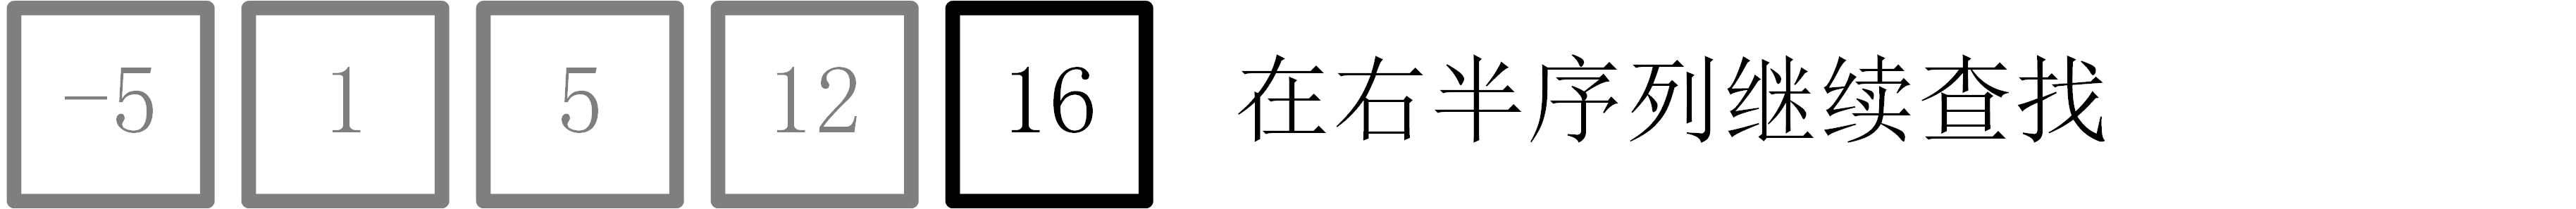
\includegraphics[width=0.8\textwidth]{binary_search_5}}\\\vspace{-10.mm}
\uncover<7->{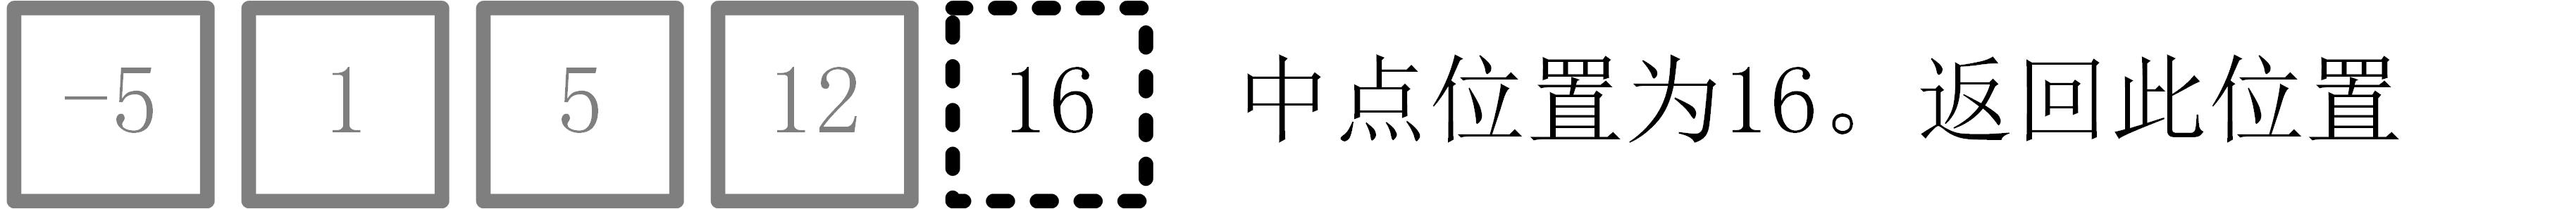
\includegraphics[width=0.8\textwidth]{binary_search_6}}\\\vspace{12mm}
\uncover<8->{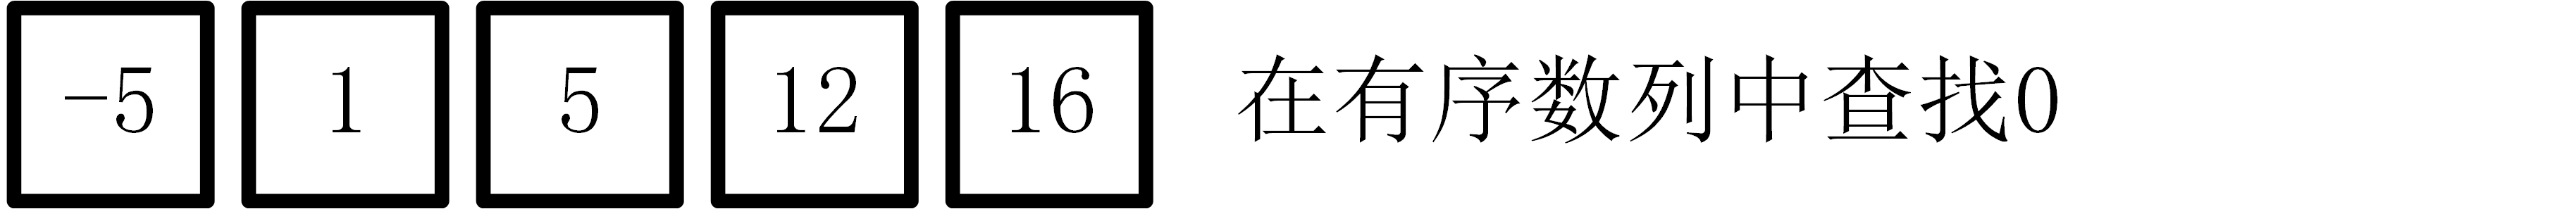
\includegraphics[width=0.8\textwidth]{binary_search_7}}\\\vspace{3mm}
\uncover<9->{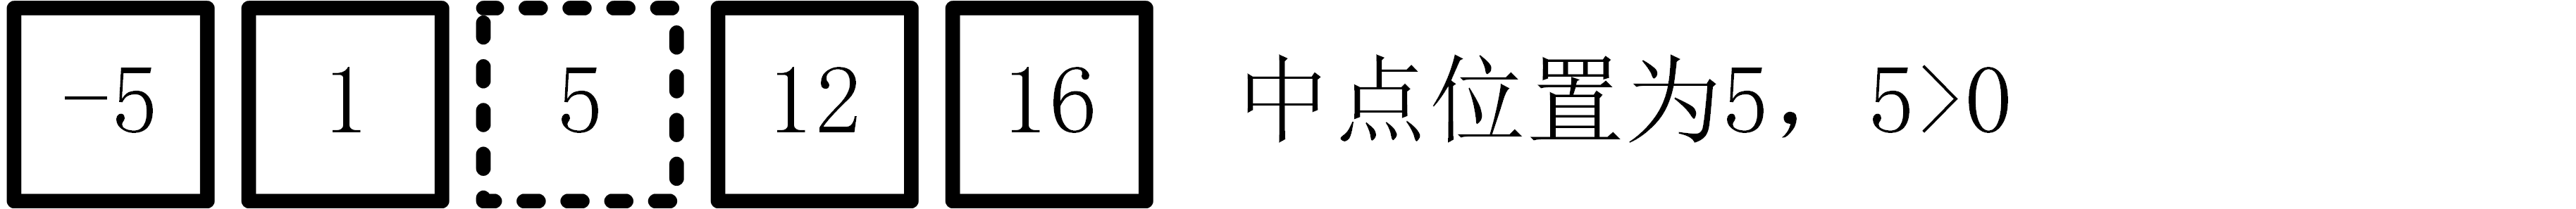
\includegraphics[width=0.8\textwidth]{binary_search_8}}\\\vspace{-10.mm}
\uncover<10->{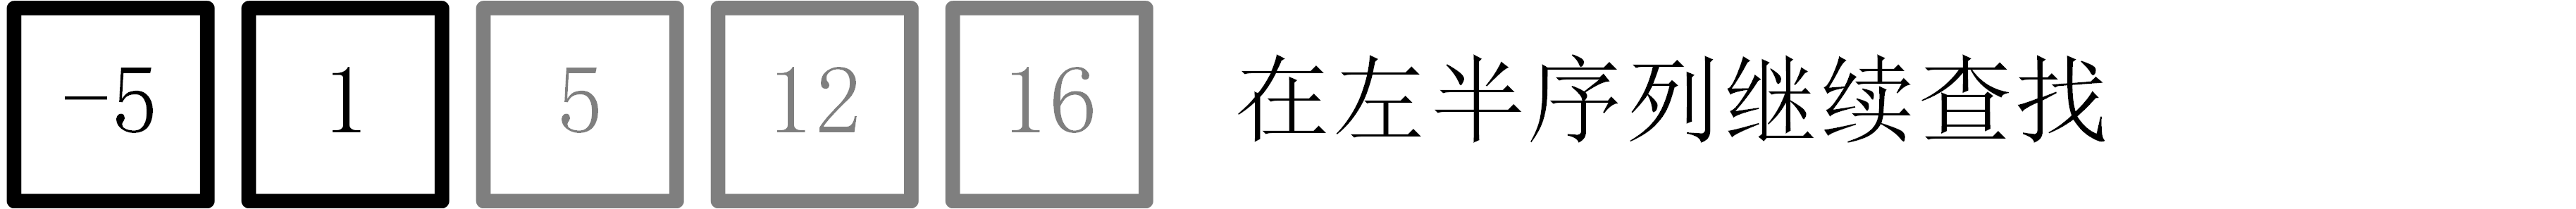
\includegraphics[width=0.8\textwidth]{binary_search_9}}\\\vspace{-10.mm}
\uncover<11->{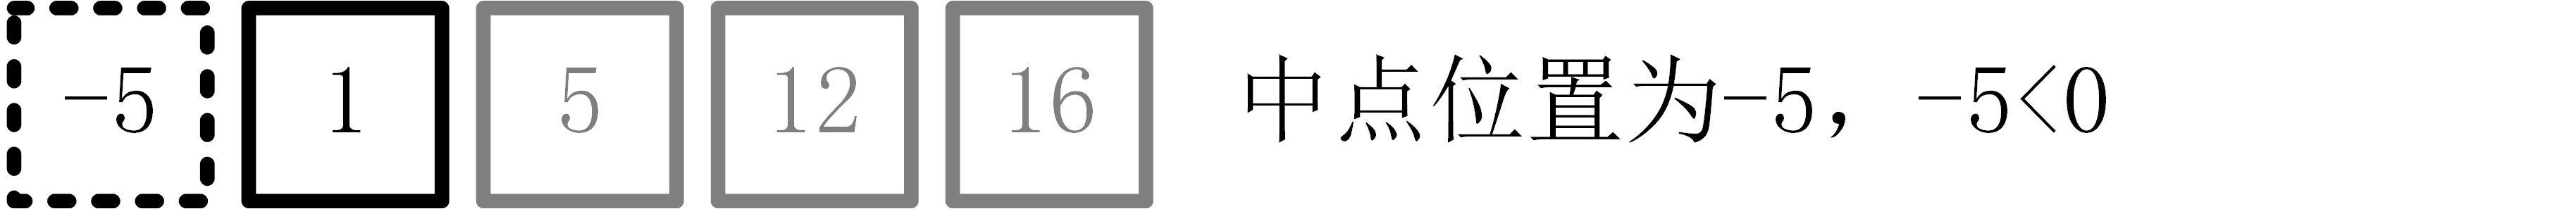
\includegraphics[width=0.8\textwidth]{binary_search_10}}\\\vspace{-10mm}
\uncover<12->{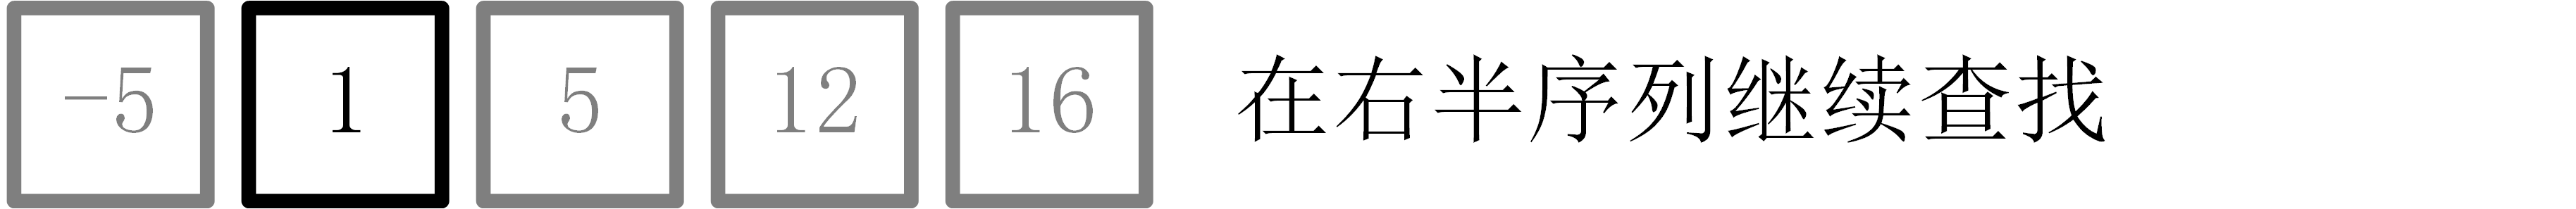
\includegraphics[width=0.8\textwidth]{binary_search_11}}\\\vspace{-10.mm}
\uncover<13->{\includegraphics[width=0.8\textwidth]{binary_search_12}}\\\vspace{-10.mm}
\uncover<14->{\includegraphics[width=0.8\textwidth]{binary_search_13}}\\\vspace{-10.mm}
\uncover<15->{\includegraphics[width=0.8\textwidth]{binary_search_14}}\\\vspace{-10.mm}
\end{center}

\end{frame}

%-----------------

\begin{frame}[fragile]{7.3.2~二分查找算法}

二分查找算法的实现如下:

\vspace{-4mm}

\begin{columns}[t]

\column{0.65\textwidth}
\begin{blueblock}{\texttt{Array}成员函数\texttt{binarySearch}定义}
\begin{lstlisting}[moreemph={Array,T,F}]
template<typename T, size_t N>
int Array<T, N>::binarySearch(const T &value, int left, int right) {
    while (left <= right) {
        int middle = (left + right) / 2;    //计算中点位置
        if (m_ele[middle] == value)
            return middle;
        else if (m_ele[middle] > value)
            right = middle - 1;             //修改right
        else
            left = middle + 1;              //修改left
    }
    return -1;                              //查找失败
}
\end{lstlisting}
\end{blueblock}


\column{0.3\textwidth}
\begin{yellowblock}{说明}
$\bullet$ \texttt{value}小于中点位置元素,将\texttt{right}设为\texttt{middle-1}\\
$\bullet$ \texttt{value}大于中点位置元素,将\texttt{left}设为\texttt{middle+1}\\
$\bullet$ 查找失败则返回\texttt{-1}
\end{yellowblock}
\vspace{-2mm}
\begin{greenblock}<2->{问题}
查找\texttt{4}返回时,\texttt{left}和\texttt{right}的值是多少?
\end{greenblock}
\vspace{-2mm}
\begin{greenblock}<3->{答案}
\texttt{left}为\texttt{2},\texttt{right}为\texttt{1}
\end{greenblock}

\end{columns}

\end{frame}

%-----------------

\begin{frame}[fragile]{7.3.2~改进插入排序算法效率}

\begin{greenblock}{问题}
如何改进插入排序算法的效率?
\end{greenblock}

\end{frame}
